\documentclass[letterpaper, 12pt]{article}
\usepackage[top = 1.6cm, left = 2cm, right = 2cm ]{geometry}
\usepackage[pdftex]{graphicx}
\usepackage{soulutf8}
\usepackage{amsmath}
\usepackage{tikz}
\usepackage[utf8]{inputenc}
\usepackage{longtable}
\usepackage[T1]{fontenc}
\usepackage{epigraph}
\usepackage{fancyhdr}
\usepackage{float}
\usepackage{subfig}
\usepackage{xcolor}
\usepackage{eurosym}
\usepackage{calc}
\usepackage{multirow} 
%
%
%%%%% Custom commands
%
%
\def\changemargin#1#2{\list{}{\rightmargin#2\leftmargin#1}\item[]}
\let\endchangemargin=\endlist 
%
\newcommand{\newlinealinea}{
~\\ \hspace*{0.5cm}}
%
\newcommand{\alinea}{
\hspace*{0.5cm}}
%
\newcommand{\alinealong}{
\hspace*{1.1cm}}
%
\newcommand{\alignparagraph}{
\hspace*{0.6cm}}
%
\newcommand{\red}[1]{
	\textcolor{red}{#1}}
%
\newcommand{\green}[1]{
	\textcolor{green}{#1}}
%
\newcommand{\point}{$\bullet\ $}
%
\makeatletter
	\newcommand*{\whiten}[1]{\llap{\textcolor{white}{{\the\SOUL@token}}\hspace{#1pt}}}
	\newcommand{\myul}[1]{
		\underline{\smash{#1}}
	}
\makeatother
%
\setlength{\fboxsep}{2pt}
%
\DeclareMathOperator*{\argmax}{\arg\!\max}
%
%
%%%%% Custom text
%
%
\makeatletter
\@addtoreset{section}{part}
\makeatother  
%
\renewcommand*\sfdefault{phv}
\renewcommand*\rmdefault{ppl}
%
\renewcommand\epigraphflush{flushright}
\renewcommand\epigraphsize{\normalsize}
\setlength\epigraphwidth{0.7\textwidth}
%
\definecolor{titlepagecolor}{cmyk}{0.24,0.92,0.78,0.25}
\definecolor{red}{cmyk}{0, 0.91, 0.91, 0.20}
%
\DeclareFixedFont{\titlefont}{T1}{phv}{\seriesdefault}{n}{0.375in}
%
%
%%%%% Header
%
%
\pagestyle{fancy}
\lhead{Anthony Rouneau}
\rhead{MAB1 Sciences Informatiques}
\cfoot{\thepage}
%
%
%%%%% Title page. The following code is borrowed from: 
%%%%%       http://tex.stackexchange.com/a/86310/10898
%
%
\newcommand\titlepagedecoration{%
\begin{tikzpicture}[remember picture,overlay,shorten >= -10pt]

\coordinate (aux1) at ([yshift=-70pt]current page.north east);
\coordinate (aux2) at ([yshift=-460pt]current page.north east);
\coordinate (aux3) at ([xshift=-6cm]current page.north east);
\coordinate (aux4) at ([yshift=-150pt]current page.north east);

\begin{scope}[titlepagecolor!40,line width=12pt,rounded corners=12pt]
\draw
  (aux1) -- coordinate (a)
  ++(225:5) --
  ++(-45:5.1) coordinate (b);
\draw[shorten <= -10pt]
  (aux3) --
  (a) --
  (aux1);
\draw[opacity=0.6,titlepagecolor,shorten <= -10pt]
  (b) --
  ++(225:2.2) --
  ++(-45:2.2);
\end{scope}
\draw[titlepagecolor,line width=8pt,rounded corners=8pt,shorten <= -10pt]
  (aux4) --
  ++(225:0.8) --
  ++(-45:0.8);
\begin{scope}[titlepagecolor!70,line width=6pt,rounded corners=8pt]
\draw[shorten <= -10pt]
  (aux2) --
  ++(225:3) coordinate[pos=0.45] (c) --
  ++(-45:3.1);
\draw
  (aux2) --
  (c) --
  ++(135:2.5) --
  ++(45:2.5) --
  ++(-45:2.5) coordinate[pos=0.3] (d);   
\draw 
  (d) -- +(45:1);
\end{scope}
\end{tikzpicture}%
}
%
\begin{document}
	\begin{titlepage}
	%
	\noindent
	%
	\newgeometry{bottom = 2cm, top = 2.5cm}
	\begin{center}
		
\includegraphics[scale=1.2]{Images/UMONS}\\
			\vspace*{0.3cm}
		
\includegraphics[scale=0.23]{Images/FS_Logo}\\
			\vspace*{2.5cm}
		%
		\titlefont Résumé de Datamining et Datawarehousing \par
		%
	\end{center}
	\vspace*{3cm}
	\hfill
	%
	\begin{minipage}{0.18\linewidth}
		\begin{flushright}
			\rule{0.5pt}{50pt}
		\end{flushright}
	\end{minipage}
	%
	\begin{minipage}{0.8\linewidth}
		\begin{flushleft}
			\textsf{\textbf{Résumé realisé par:}} Anthony Rouneau\\
			\textsf{\textbf{Section:}} 1$^{er}$ Bloc Master en 
				Sciences Informatiques
		\end{flushleft}
	\end{minipage}
	%
	\vspace*{\fill}                                                             
	%
	\begin{center}
		Faculté des Sciences $\bullet$ Université de Mons $\bullet$ 
		Place du Parc 20 $\bullet$ B-7000 Mons
	\end{center}
	%
	\titlepagedecoration
	%
\end{titlepage}
%
%
%%%% Tables des matières
%
%
\newgeometry{top = 3cm, left = 2cm, right = 2cm, bottom=2.5cm}
%
\tableofcontents
%
\newpage
%
%
\part{Classification}
	\alinea Le rôle d'une classification est d'assigner des objets
		(instances) à
		une classe selon une suite d'attributs. Chaque objet peut donc
		être représenté par un tuple $(x, y)$, où $x$ est une séquence
		d'attributs et $y$ le nom de sa classe.\\
	%
	\alinea Un \myul{\textbf{attribut}} peut être discret ou continu,
		contrairement au \myul{\textbf{label de classe}}, 
		qui lui doit être discret. Ce qui
		veut dire que le nombre de classes dans lesquelles les instances
		seront classé est fini, et que toutes les classes sont à priori
		connues. \hl{C'est ce qui différencie une classification d'une 
		régression}\\
	%
	~\\
	%
	\myul{\textbf{Classification}}-- \red{Tâche de construire/%
		d'apprendre une fonction $f$ qui fera correspondre un ensemble
		d'attributs, un objet, $x$ à une des classes prédéfinies, $y$.}
	%
	\paragraph{\point Buts d'une classification}~\\~\\
	%
	\begin{tabular}{lp{11cm}}
	    \myul{\textbf{Modélisation descriptive}}& 
	    	\red{Utilisation d'une classification dans le but de lister les
			attributs qui définissent une certaine classe.}
			(e.g. attributs d'animaux $\rightarrow$ famille d'animaux.\\
	    \myul{\textbf{Modélisation prédictive}}&
			\red{Utilisation d'une classification pour prédire la classe
			d'objets inconnus.} Notons qu'une classification n'est pas
			performante pour des classes ordonnées (avec une hiérarchie
			ou un ordre définie).
	\end{tabular}				
	%
	\section{Approche générale}
		\alinea Une technique de classification consiste à construire un
			\myul{modèle} de classification depuis un 
			\myul{\textbf{ensemble de données d'entraînement}}. Ce modèle
			peut ensuite être évalué en y faisant passer un 
			\myul{\textbf{ensemble de données de test}}, idéalement 
			\hl{différent de l'ensemble d'entraînement pour éviter 
			l'\textit{overfiting}} (voir plus loin).\\
		%
		\alinea Un modèle est évalué selon plusieurs métriques,
			dont par exemple la \textit{Précision} et le 
			\textit{Taux d'erreur}.
			\begin{figure}[H]
				\centering
				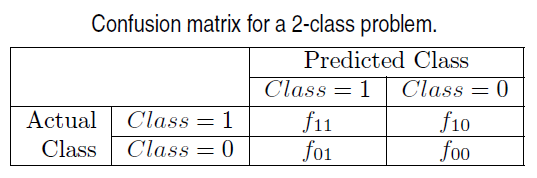
\includegraphics[scale=0.75]{Images/conf_matrix.png}
			\end{figure}\noindent
			\begin{align*}
			\text{Précision} &=& 
			\frac{\text{Nombre de prédictions correctes}}%
			{\text{Nombre total de prédiction}} &=& \frac{f_{11} + f_{00}}%
			{f_{11} + f_{10} + f_{01} + f_{00}}\\
			%			
			\text{Taux d'erreur} &=& 
			\frac{\text{Nombre de prédictions fausses}}%
			{\text{Nombre total de prédiction}} &=& \frac{f_{10} + f_{01}}%
			{f_{11} + f_{10} + f_{01} + f_{00}}\\
			\end{align*}%
		%
	%
	\section{Arbre de décision (DTI)}
		\begin{center}DTI = Decision Tree Induction.\end{center}
		\alinea Le nombre d'arbres de décision pouvant découler d'un ensemble
			d'attributs est exponentiel. Il est donc impossible de trouver
			l'arbre optimal pour un problème de classification donné.
			C'est pourquoi \hl{la plupart des techniques de construction 
			utilisent un algorithme glouton (greedy)}.
		%
		\subsection{Algorithme de Hunt}
			\alinea Les méthodes de construction \texttt{ID3}, \texttt{C4.5},
				\texttt{CART} découlent
				toutes du même algorithme : l'algorithme de Hunt. 
				L'algorithme consiste à partitionner récursivement 
				les données d'entraînement dans de sous-ensembles plus
				"purs". Celui-ci est décrit ci-dessous.\\
			%
			~\\
			%
			\alinea Soit $D_t$ le sous-ensemble des données 
				d'entraînement qui est associés au noeud $t$ de l'arbre, et 
				$y=\{y_1,y_2, \ldots, y_c\}$ les labels de classe.\\
			%
			~\\
			%
			\begin{tabular}{lp{15.5cm}}
			\myul{\textbf{\'Etape 1}} & \red{Si tous les objets de $D_t$
				appartiennent 
				à la même classe $y_t$, alors, le noeud $t$ est une feuille
				avec le label $y_t$.}\\
			\myul{\textbf{\'Etape 2}} & \red{Si $D_t$ contient des instances 
				qui appartiennent
				à plus qu'à une classe, une \textbf{condition de test
				d'attribut} est sélectionnée pour partitionner les objets
				dans de plus petits sous-ensembles. Un noeud fils est créé 
				pour chaque sortie de la condition de test et les objets
				de $D_t$ sont répartis dans les noeuds fils selon la 
				condition sélectionnée.} Pour bien partitionner, il faut
				tenir compte du type d'attribut 
				(cf. \ref{sec:tree:test_cond}) et savoir évaluer la qualité
				d'une partition (cf. \ref{sec:tree:split}).\\
			\myul{\textbf{\'Etape 3}} & \red{Recommencer jusqu'à ce qu'on
				ne doive plus diviser aucun noeud.} Il y a plusieurs méthodes
				pour déterminer cela. Soit on peut attendre qu'il n'y ait 
				plus que des feuilles parfaites, ne contenant qu'une seule
				classe chacune, soit on peut arrêter le processus plus tôt.
			\end{tabular}\noindent
			%
			~\\~\\~\\
			%
			\alinea Pour que cet algorithme fonctionne, il faudrait que
				chaque combinaison des valeurs d'attributs soit
				présente dans les données d'entraînement et que chaque 
				combinaison ait une classe unique (classification parfaite
				car on aurait géré tous les cas possibles). Ce n'est
				évidemment pas possible, c'est pourquoi \hl{les deux 
				conditions ci-dessous sont nécessaires en pratique}.
			%
			\begin{enumerate}
				\item Il est possible qu'un des noeuds fils créés à l'étape
				2 soit vide (aucune des instances ne correspond à la
				condition).
				Dans ce cas, \hl{le noeud fils vide en question devient une 
				feuille et aura comme label la classe majoritaire présent
				dans son parent.}
				%
				\item Si dans l'étape 2, \hl{tous les objets sont les même},
				mais qu'ils n'appartiennent pas à la même classe
				(contradictions, bruits), il n'est dés lors plus 
				possible de diviser le noeud.
				\hl{Il deviendra donc une feuille et aura comme label
				la classe majoritairement représentée par ses objets.}
			\end{enumerate}
			%
		%
		\subsection{Choisir la condition de test}\label{sec:tree:test_cond}
			\alinea Il faut pouvoir diviser les différents attributs en
				fonction de leur type.
			%
			\paragraph{Attributs binaire} La condition de test génère deux
				noeuds fils, un par valeur possible.
			%
			\paragraph{Attributs nominaux} Les deux manières de division
				sont illustrées par la figure \ref{fig:tree:nominal}. 
				\hl{\`A savoir que des algo. de construction d'arbres, comme
				\texttt{CART} ne produise que des sorties binaires}, en
				choisissant la meilleure découpe binaire parmi les
				$2^{k-1} -1$ possibilités.\\
				%
				\begin{minipage}{0.45\textwidth}
					\begin{figure}[H]
						\centering
						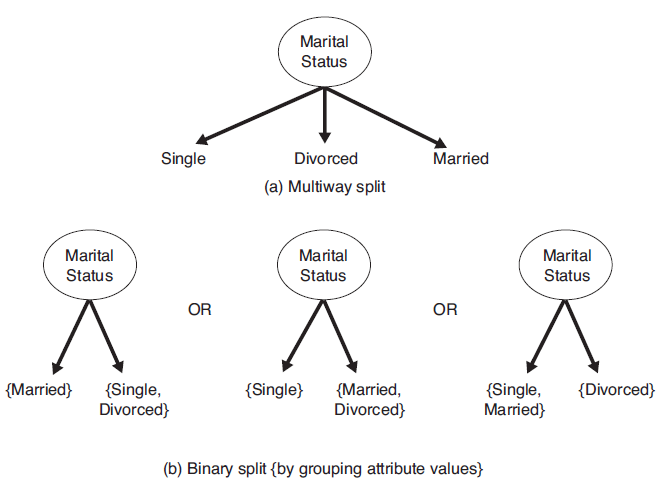
\includegraphics[scale=0.65]{Images/tree_nominal.png}
						\caption{Division d'attributs nominaux}
						\label{fig:tree:nominal}
					\end{figure}\noindent
				\end{minipage}\hfill
				\begin{minipage}{0.45\textwidth}
					\begin{figure}[H]
						\centering
						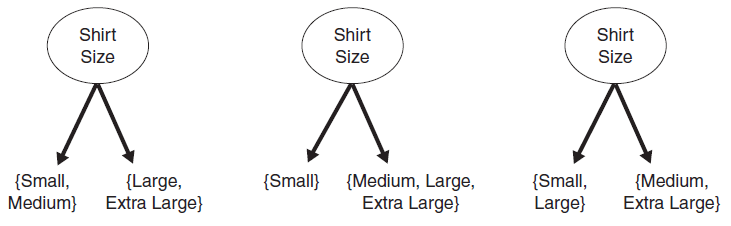
\includegraphics[scale=0.6]{Images/tree_ordinal.png}
						\caption{Division d'attributs ordonnés}
						\label{fig:tree:ordinal}
					\end{figure}\noindent
					\begin{figure}[H]
						\centering
						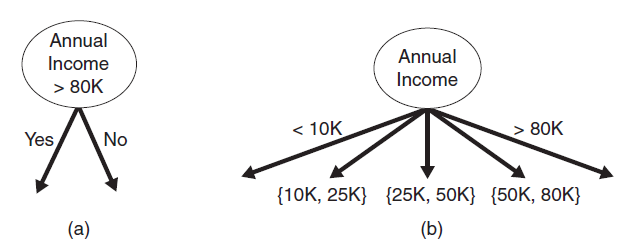
\includegraphics[scale=0.6]{Images/tree_continuous.png}
						\caption{Division d'attributs continus}
						\label{fig:tree:continuous}
					\end{figure}\noindent
				\end{minipage}
				%
			%
			\paragraph{Attributs ordonnés} De la même manière que les 
				nominaux, \hl{tant que l'ordre des attributs n'est pas
				cassé par les partitions}, voir la figure
				\ref{fig:tree:ordinal}.
			%
			\paragraph{Attributs continus} Même chose que les deux derniers,
				même si cette fois, on a une condition sur la valeur
				continue, comme représenté sur la figure
				\ref{fig:tree:continuous}. L'algorithme va
				évaluer les différents splits possibles et choisir le
				meilleur. Pour une division \textit{multiway}, 
				une discrétisation est généralement opérée sur les valeurs
				des attributs.
			%
		%
		\newpage
		%
		\subsection{Qualité d'un partitionnement}\label{sec:tree:split}
			\alinea Pour évaluer la qualité d'un partitionnement, définissons
				$p(i|t)$ comme étant le \textbf{pourcentage} (entre 0 et 1)
				d'objets appartenant à
				la classe $i$, pour un noeud d'arbre $t$. Quand le noeud
				n'est pas utile, la notation peut se réduire à $p_i$.
				Pour une classe binaire, $(p_0, p_1)$ peut-être utilisé
				avec $p_1 = 1 - p_0$.
			%
			\paragraph{\point Impureté d'un noeud}~\\~\\
			%
			\alinea Plus une classe est majoritairement représentée par les 
				objets du noeud, au plus ce noeud, cette partition, sera
				considérée comme \textit{pure}. En pratique, c'est le degré
				d'impureté qui sera mesuré. un noeud $(0, 1)$ n'a aucune 
				impureté, tandis qu'un noeud $(0.5, 0.5)$ est le plus impur
				possible (aucune classe n'est majoritairement représentée).\\
			%		
			\alinea Quelques \hl{exemples de mesures d'impuretés} ($c$
				= le nombre de classes différentes, et $0log_20 = 0$
				pour le calcul de l'\textit{Entropy}) :
			\begin{align*}
				\text{Entropy}(t) &= -\sum^{c-1}_{i=0} p(i|t) 
					\cdot log_2 (p(i|t))\\
				\text{Gini}(t)    &= 1- \sum^{c-1}_{i=0}[p(i|t)]^2\\
				\text{Classification error}(t) &= 1-\max_{i}[p(i|t)]
			\end{align*}
			%
			\alinea Les trois mesures, bien que différentes, respecte
				toutes la mesure "d'impureté" et ont donc le même pire cas
				et le même meilleur cas. Cependant, la mesure choisie peut
				influencer le résultat du partitionnement.
			%
			\paragraph{\point Impureté d'un split}~\\~\\
			% 
				\alinea Pour évaluer 
				l'impureté d'un partitionnement, on va utiliser une
				moyenne pondérée par rapport au nombre d'objet
				par partition.
				$$ I(\text{split}) = \sum_{j=1}^{k}\frac{N(v_j)}{N} 
					I(v_j) $$
				Avec $I$ la mesure d'impureté, $k$ le nombre de partitions,
				$N$ le nombre total d'objets, et $N(v_j)$ le nombre d'objets
				présents dans la partition (noeud fils) $v_j$.
			%
			\begin{figure}[H]
				\centering
				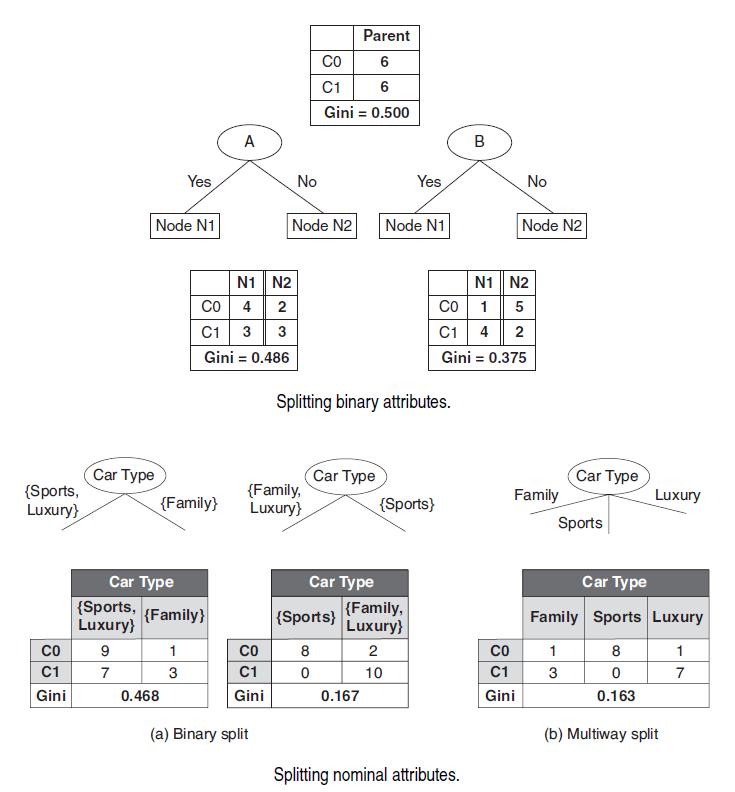
\includegraphics[scale=0.8]{Images/tree_split_measure.png}
				\caption{Exemple de $\text{Gini}(\text{split})$ de
						 partitionnements d'attributs 
						 binaires et nominaux}
				\label{fig:tree:split_measure}
			\end{figure}\noindent
			%
			Par exemple, prenons la figure \ref{fig:tree:split_measure},
			le tableau \texttt{Car Type} ((b), split \textit{multiway}).
			Le calcul se fait comme suit ($\{value\}$ représentant un 
			noeud fils, une partition) : 
			\begin{align*}
				\text{Gini}(\text{split}) &= \frac{4}{20} \cdot 
					\text{Gini}(\{\text{Family}\}) + \frac{8}{20} \cdot 
					\text{Gini}(\{\text{Sports}\}) + \frac{8}{20} \cdot 
					\text{Gini}(\{\text{Luxury}\})\\
				%
				\text{Gini}(\text{split}) &= 
				\frac{4}{20} \cdot 
				[1 - (\sum_{i=0}^{1}[p(C_i|\{\text{Family}\})]^2] + 
				\frac{8}{20} \cdot 
				[1 - (\sum_{i=0}^{1}[p(C_i|\{\text{Sports}\})]^2]\\ 
				&+ 
				\frac{8}{20} \cdot 
				[1 - (\sum_{i=0}^{1}[p(C_i|\{\text{Luxury}\})]^2])\\
				%
				\text{Gini}(\text{split}) &= \frac{4}{20} \cdot 0.375
					 + \frac{8}{20} \cdot 0
					 + \frac{8}{20} \cdot 0.163 = 0.163
			\end{align*}
			C'est normal que le \textit{multiway} ait de meilleurs résultats
				que les binaires, car faire du binaire, c'est en quelques
				sorte fusionner	des résultats de \textit{multiway}\\	
			%
			\begin{figure}[H]
				\centering
				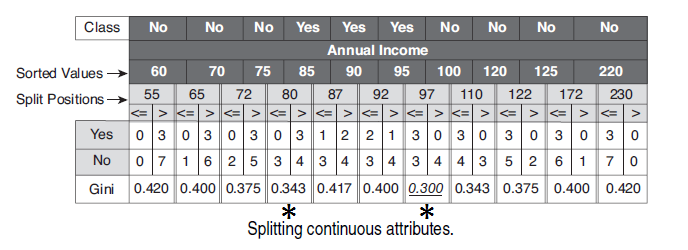
\includegraphics[scale=1.0]{Images/tree_split_measure2.png}
				\caption{Exemple de Gini$($split$)$ d'un partitionnement
						 d'attribut continu}
				\label{fig:tree:split_measure2}
			\end{figure}\noindent
			%
			\alinea En ce qui concerne les attributs continus, 
				il faut réduire 
				le nombre de calculs pour décider du meilleur split. 
				Regardons la figure \ref{fig:tree:split_measure2}.
				\hl{Pour réduire les calculs, on va classer les objets 
				par leur valeur d'attribut
				(Sorted Values). Ensuite, on choisit des positions de split
				en prenant des points à égales distances de deux 
				valeurs ordonnées} (Split Positions, 
				$\lfloor\frac{70 + 75}{2}\rfloor = 72$). \hl{On calcule 
				ensuite
				comme précédemment la valeur de Gini pour chaque split
				 possible},
				et le split en 97 est le meilleur par sa moyenne pondérée 
				d'impureté de 0.300.\\
			%
			\alinea \hl{On pourrait encore améliorer ceci en ne calculant 
				l'impureté que des positions de split se trouvant à la
				frontière de deux classes}. On ne garderait alors que 
				les position marqués par des $\ast$, ce qui réduit 
				considérablement les calculs.
			%			
			\paragraph{\point Gain}~\\~\\
			%
			\alinea Les algorithmes de construction d'arbres choisissent 
				généralement une fonction qui maximise \hl{le gain ($\Delta$)}, 
				c'est-à-dire qui choisisse le partitionnement qui
				améliore le plus la pureté du split comparé à la pureté
				du parent.
				$$ \Delta = I(\text{parent}) - I(\text{split}) $$
			%
			Avec $I$ la mesure d'impureté. Lorsque $I$ 
			correspond à l'\textit{Entropy}, le gain est appelé gain 
			d'information ($\Delta_{\text{info}}$). On remarque que
			\hl{maximiser $\Delta$ revient à minimiser la moyenne pondérée de 
			l'impureté des noeuds fils}.
			%
			\newpage
			%
			\paragraph{\point Ratio de gain}~\\~\\
			%
			\alinea Il peut arriver qu'un attribut soit inapproprié à
				la classification. Typiquement, on retrouve souvent un 
				attribut "ID" dans les tables. Chaque objet ayant un
				ID unique, l'attribut ne peut en aucun cas aider à la
				classification. De manière générale, on voudrait éviter
				qu'un attribut ne divise l'arbre en trop de branches.\\
			%
			\alinea Pour éviter ceci, il y a deux manières de faire :
			\begin{enumerate}
				\item Se restreindre à des splits binaires
				\item Prendre en compte dans le score d'un split le nombre 
					de partitions, comme le fait par exemple le 
					\textbf{Gain ratio}.
			\end{enumerate}
			$$ \text{Gain ratio} = \frac{\Delta_{\text{info}}}%
				{\text{Info}(split)}$$
			Ou Info$(split) = -\sum_{i=1}^{k} \frac{N(v_i)}{N} \cdot log_2
				(\frac{N(v_i)}{N})$. \hl{L'idée est que si le split a 
				beaucoup de branches, alors Info$(split)$ sera grand,
				réduisant ainsi son \textit{Gain ratio}.}
			%
		%
		\subsection{Algorithme}
			\begin{figure}[H]
				\centering
				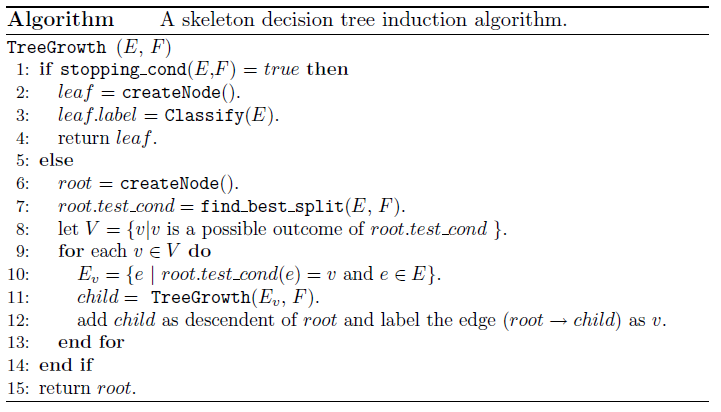
\includegraphics[scale=0.8]{Images/tree_algo.png}
				\caption{}\label{fig:tree:algo}
			\end{figure}\noindent
			%			
			\verb|Classify()| consiste à chercher un label à 
			la feuille. Dans la plupart des cas, cela consiste à faire:
			$$leaf.label = \argmax_{i}{p(i|t)}$$
			\hl{$p(i|t)$ peut dés lors être utilisé comme la probabilité
			qu'à un objet du noeud $t$ d'appartenir à la classe $i$.}\\
			%
			\alinea Après être passé dans l'algorithme, la taille de l'arbre
				peut-être réduite grâce à une étape d'élagage (pruning),
				car les arbres trop larges font souvent l'objet
				d'\textit{overfitting}.
			%
		%
		\subsection{Caractéristiques}
			\alinea Les caractéristiques principales d'une classification
				par arbre de décision sont les suivantes:
			\begin{enumerate}
				\item Technique non-paramétrique. Aucune hypothèse sur le
					jeu de donnée n'est nécessaire.
				\item La recherche de l'arbre optimale $\in NP-Complet$,
					les méthodes utilisées sont des heuristiques.
				\item Les techniques développées sont très rapides 
					d'exécution.
				\item Un arbre est facile à interpréter et à comparer
					à d'autres modèles.
				\item Donne une représentation expressive pour l'apprentissage
					de fonctions à valeurs discrètes. \hl{Même s'il y a
					quelques exceptions avec des problèmes Booléens, comme
					la fonction de parité, dont la valeur est 0
					(\textit{resp.} 1) quand il y a un nombre impair 
					(\textit{resp.} pair) d'attribut Booléen. Il faut
					un arbre complet avec $2^d$ noeud ($d$ = nbre d'attribut
					Booléen) pour avoir un arbre permettant de répondre.}
				\item Les arbres sont robustes au bruit.
				\item Les \textbf{attributs redondants} ne posent pas 
					de problèmes. Un attribut est redondant lorsqu'il y a une
					forte corrélation entre cet attribut et un autre.
					\hl{En pratique, quand l'un des deux attributs redondants
					sera utilisé pour un split, l'autre ne sera pas utilisé.}
					Si l'arbre est trop grand, il se peut qu'il y ait tout
					de même des splits redondant, qui seront coupé à l'élagage.
				\item Si une feuille contient trop peu d'objets, on parle
					de \textbf{fragmentation des données}. On peut l'éviter
					en refusant de split lorsqu'on a plus assez d'objets.
				\item Des sous-arbres peuvent être dupliqué dans l'arbre
					de décision. Ceux-ci seront fusionnés dans l'élagage.
				\item Les frontières, formées par les attributs (cf. figure
					\ref{fig:tree:boundaries}), 
					entre les classes sont rectilignes pour les arbres car
					l'étape de division se fait pour un attribut à la fois,
					ce qui empêche de trouver les relations complexes qu'il
					peut y avoir entre les attributs. Des \textbf{arbres
					de décision obliques} peuvent être utilisés pour 
					résoudre ce problème, ils prennent plus qu'un attribut
					pour diviser leurs attributs, ce qui multiplie les
					calculs... Il existe aussi la \textbf{construction 
					inductive}, qui va créer de nouveaux attributs à partir
					des attributs de base qui sont liés entre eux. \hl{Ceci 
					demande moins de calcul car les relations entre
					attributs se calculent une seule fois.}
				\item Le choix de l'impureté n'a pas beaucoup d'influence
					sur la qualité de l'arbre final. \hl{La stratégie
					d'élagage, par contre, peut l'influencer.}
			\end{enumerate}
			%
			\begin{figure}[H]
				\centering
				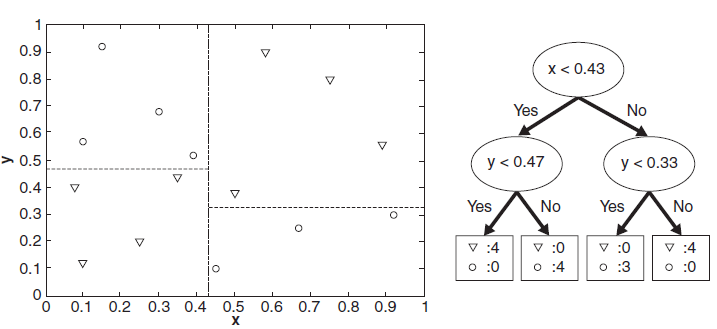
\includegraphics[scale=0.75]{Images/tree_boundaries}
				\caption{Exemple de frontières séparant les classes}
				\label{fig:tree:boundaries}
			\end{figure}\noindent
			%
			\begin{figure}[H]
				\centering
				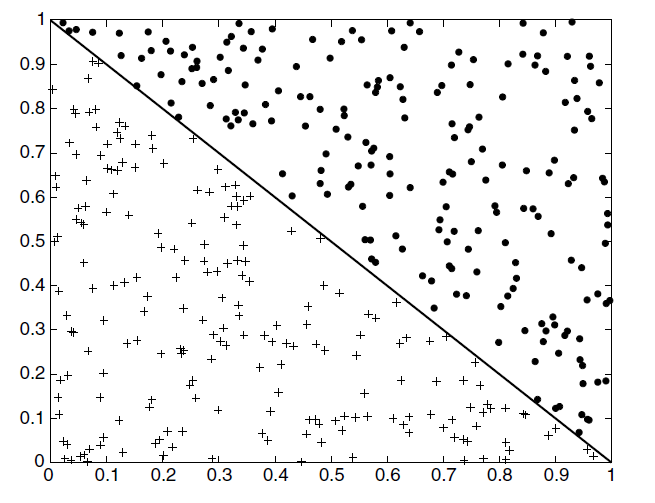
\includegraphics[scale=0.45]{Images/one_rule.PNG}
				\caption{\hl{Exemple de jeu de donnée ne pouvant pas
				être classé}} 
				\hl{en n'utilisant que des conditions sur 
				des attributs\\ simple (il faudrait utiliser plusieurs
				attributs)}
				\label{fig:one_attribute}
			\end{figure}\noindent
			%
		%
	%
	\section{Overfitting}
		On divise les erreur de classification en deux types 
			d'erreur : \\
			\begin{enumerate}
				\item \myul{\textbf{\hl{Les erreurs d'entraînement,
				    ou erreurs de resubstitution}}}--
				 \red{Erreurs commises sur les données d'entraînement.}
				\item \myul{\textbf{\hl{Les erreurs de généralisation}}}--
				 \red{Erreurs commises sur des données données extérieures,
					ne venant pas du jeu d'entraînement.}
			\end{enumerate}
		%
		\alinea Dans les deux cas, l'erreur représente le nombre d'objets
			mal classifiés sur le nombre total d'objet du jeu de données.\\
		%
		~\\
		%
		\alinea Un modèle présentant plus d'erreur de généralisation 
			que d'erreur
			d'entraînement est ce qu'on appel un modèle qui fait de
			l'\hl{\textit{overfitting}}, c'est-à-dire qu'il colle trop à ses
			données d'entraînement et qu'il n'est pas très bon pour classer
			d'autres objets, même s'il esst peut-être bon pour les données
			d'entraînement. \\
		%
		\alinea Lorsqu'un modèle est trop restreint, il peut y avoir
			le phénomène d'\textit{\hl{underfitting}} qui apparaît.
			Ceci veut dire que le modèle n'a pas saisi les caractéristiques
			qui permettent de classifier correctement et est donc mauvais
			à la fois pour classer les données d'entraînement, mais aussi
			pour classer les données extérieures.
		%
		\subsection{Bruit}
			\alinea Le bruit est une des causes dee l'\textit{overfitting}.
				Si par exemple des objets sont mal classifiés dans le jeu de 
				données d'entraînement, cela va induire en erreur le modèle
				et peut donc commettre cette erreur en essayant de classifier
				des données extérieures.\\
			%
			\alinea On peut parfois identifier la partie du modèle
				qui pose problème, et la supprimer.
			%
		%
		\subsection{Manque de représentativité}
			\alinea Si il y a un petit nombre d'objets, ou du moins, 
				qu'une classe compte un petit nombre d'objets dans le
				jeu de données d'entraînement, le modèle
				va avoir du mal à identifier ce qui caractérise cette 
				classe mal représentée (e.g. 5 $no$, 1 $yes$).
			%
		%
		\subsection{Procédure de comparaison multiple}
			\alinea Pour illustrer ce qu'est la comparaison multiple,
				imaginons qu'on doive prédire s'il va pleuvoir demain.
				Si on tire au hasard, la probabilité qu'on ait raison
				est de 0.5. Par contre, si on doit prédire pour les 
				dix prochains jour, la probabilité qu'on ait raison
				au moins 8 fois sur 10 est de :
				$$ \frac{\binom{10}{8} + \binom{10}{9} + \binom{10}{10}}%
						{2^{10}} = 0.0547 $$
			%			
			\alinea Ce n'est pas très élevé, mais si on demande à 50
				personnes de faire le même travail pour les 10 jours à venir,
				$Nobody$ étant la probabilité que personne n'ait raison
				au moins pour 8 jours, et $AtLeastOne$ la probabilité qu'au
				moins une des 50 personnes ait raison 8 fois sur 10 :
				$$ Nobody = (1-0.0547)^{50} $$
				$$ AtLeastOne = 1 - Nobody = 0.9399 $$
			%
			\alinea Mais même si l'on trouve la personne qui a trouvé, 
				rien ne garanti que cette même personne est douée dans
				ce qu'elle fait. Peut-être qu'elle a juste deviné au hasard, 
				huit jours de suite.\\
			%
			\alinea On peut faire l'analogie avec la construction d'un arbre
				de décision. Si l'on dit qu'on a un arbre $T_0$ et qu'on
				cherche, parmi $k$ splits différents du noeud courant, 
				$T_{x_{max}}$, l'arbre résultant de l'ajout du split, de
				gain maximum.\hl{ Et si l'on dit que l'on choisit $T_{x_{max}}$
				pour continuer plutôt que $T_0$ si ce gain dépasse un 
				seuil $\alpha$ ($\Delta(T_0, T_{x_{max}}) > \alpha$).
				Et bien plus $k$ augmente, plus on a de chance de trouver 
				le split qui va donner un gain assez élevé}. Mais 
				si le nombre de donnée est réduit, la variance de ce gain
				est plus grand, et il y a de grandes chances qu'un gain
				"hasardeux" soit choisi car il dépassait $\alpha$ (à l'image
				du météorologiste chanceux, on a aucune garantie que cet
				ajout au modèle restera performant pour les données
				extérieures).
			%
		%
		\subsection{Estimation des erreurs de généralisation}
			\alinea La complexité d'un modèle influence l'\textit{overfitting}.
				\hl{La question est donc quelle est la complexité idéale pour
				un modèle ?} Il faudrait minimiser le taux d'erreur de 
				généralisation, mais lors de la création du modèle, 
				l'algorithme n'a accès qu'aux données d'entraînement.
			%
			\subsubsection{Estimation par resubstitution}
			%
			\alinea On suppose ici que le jeu de données d'entraînement
				représente bien les données globales du problème. Il suffit
				donc de minimiser l'erreur d'entraînement pour minimiser,
				par hypothèse, l'erreur de généralisation. 
				\red{Pas bon en pratique.}
			%
			\subsubsection{Incorporation de la complexité du modèle}
			%
			\alinea Comme l'\textit{overfitting} peut venir d'un modèle
				trop complexe, préférer des modèles plus simples permettrait
				de limiter l'\textit{overfitting}, c'est le principe
				du \textbf{Rasoir d'Occam}.\\~\\
				\begin{tabular}{lp{13.5cm}}
					\myul{\textbf{Rasoir d'Occam}}-- & 
						\red{Parmi deux modèles avec la même erreur de 
							 généralisation, le modèle le plus simple des
							 deux est préféré au plus complexe.}
				\end{tabular}~\\~\\
			%
			\alinea Comme disait Einstein, \hl{"Tout devrait être fait le 
				plus simple possible, mais pas plus simple"}. Il ne faudrait
				donc pas prendre un modèle trop simple, au risque 
				d'\textit{underfitting}.\\
			%
			\alinea Ci-dessous sont présenté deux méthodes d'intégration
				de la complexité dans l'évaluation des modèles.
			%
			\paragraph{\point Estimation pessimiste de l'erreur}~\\~\\
				On additionne
				l'erreur d'entraînement et la complexité du modèle. 
				Appelons $n(t)$ le nombre d'objets d'entraînement classifié 
				par le noeud $t$ et $e(t)$ le nombre d'objet mal classifiés.
				l'estimation pessimiste de l'erreur d'un arbre $T$, $e_g(T)$
				est la suivante :
				$$ e_g(T) = \frac{\sum_{i=1}^{k}[e(t_i) + \Omega(t_i)]}%
				                 {\sum_{i=1}^{k}n(t_i)}
				          = \frac{e(T) + \Omega(T)}{N_t} $$
				Avec $k$ le nombre de feuilles, $e(T)$ 
				l'erreur globale d'entraînement, $N_t$ le nombre d'objets
				d'entraînement, et $\Omega(T)$ la pénalité associée à 
				chaque noeud $t_i$. La valeur de cette pénalité décidera
				de l'importance que l'on accorde à la complexité dans 
				l'estimation. \\
				%
				~\\				
				%
				\hl{Pour un arbre binaire, une pénalité de 0.5
				indique qu'un noeud doit toujours se diviser en deux}
				si la division permet de mieux classer au moins un objet 
				d'entraînement, en effet, ajouter une pénalité de 0.5
				à l'erreur en créant une nouvelle feuille 
				(on en crée deux, mais
				on ajoute qu'une seule feuille, étant donné que le parent 
				était précédemment une feuille, et qu'il n'en est plus une)
				est moins couteux que de commettre une erreur d'entraînement.
				\hl{Et une pénalité valant 1 indique que pour diviser un noeud,
				il faut que la division permette d'améliorer 
				la classification d'au moins deux objets d'entraînement.}
				%
			%
			\paragraph{\point Description de longueur minimal (\hl{MDL})}~\\~\\
				Approche venant de la théorie de l'information.
				En prenant la figure \ref{fig:mdl} comme exemple,
				où $A$ et $B$ partage un jeu de donnée $X$, mais où il
				n'y a que $A$ qui connait $y$.
				$A$ voudrait donc transmettre les labels ($y$)
				à $B$, ce qui représente $O(n)$ bits d'information.
				Si $A$ arrive à créer un modèle permettant de déduire
				$y_i$ de $X_i$, alors \hl{si la taille de l'encodage
				du modèle est inférieur à la taille de l'encodage
				des $y$, il est plus intéressant d'envoyer le modèle
				plutôt que $y$ en entier}.\\
				%
				~\\
				%
				Il se peut cependant que le modèle ne permettent pas une
				classification sans faute. Il faudra alors envoyer à $B$
				ces objets, mal classifiés, individuellement.
				$$ Cost(model, data) = enc(model) + enc(misclassified) $$
				\hl{$enc(model)$ étant le coût de l'envoi de l'encodage du
				modèle
				et $enc(misclassified)$ le coût de l'envoi de l'encodage
				des objets mal classifiés par le modèle.
				On devrait donc chercher un modèle qui minimise se coût.}	
				%
				\begin{figure}[H]
					\centering
					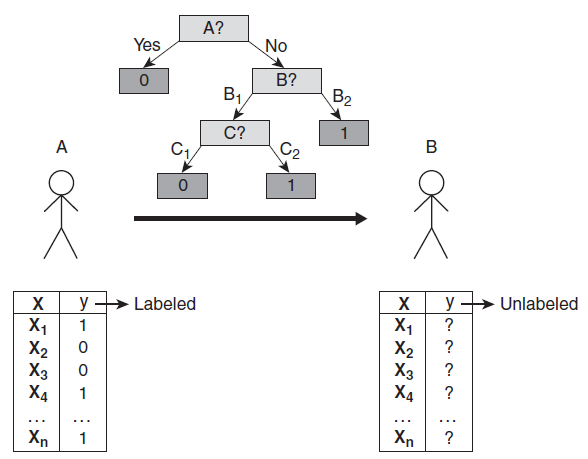
\includegraphics[scale=1.0]{Images/mdl.png}
					\caption{Minimum Description Length (MDL) Principle}
					\label{fig:mdl}
				\end{figure}\noindent
				%
			%
			\newpage
			%
			\subsubsection{Estimer les bornes statistiques}
			%
			\alinea L'erreur de généralisation peut aussi être estimée
				comme une correction statistique de l'erreur d'entraînement.
				On calculera la correction statistique comme une borne
				supérieure de l'erreur d'entraînement, en prenant en compte
				le nombre d'objet qui atteignent une feuille en particulier.
				\hl{Par exemple, l'algorithme \texttt{C4.5} suppose que
				le nombre d'erreurs commises par chaque feuille suit une
				distribution binomiale.} Il faut donc déterminer la borne 
				limite supérieure à l'erreur d'entraînement observée.
			%
			\subsubsection{Utiliser des données de validation}
			%
			\alinea Dans cette méthode, on coupe le jeu de donnée
				d'entraînement en deux. Une partie (généralement $\frac{2}{3})$
				du jeu d'entraînement original est gardé pour l'entraînement
				du modèle et le reste des données est utilisé pour estimer
				l'erreur de généralisation (comme si cette partie des données
				était composée de données extérieures). \red{Le point faible
				de cette méthode est que l'on retire des données du
				jeu d'entraînement, ce qui peut causer des lacunes dans le
				modèle (classe trop peu représentée, ...).}
			%
		%
		\subsection{Overfitting des arbres de décision}
			\alinea \hl{Avoir une estimation fiable de l'erreur 
				de généralisation
				permet à l'algorithme de classification de chercher un 
				modèle précis sans \textit{overfitter} les données d'%
				entraînement.} Ci-dessous sont présentées deux stratégies
				qui permettent d'éviter l'\textit{overfitting} dans les
				arbres de décision.
			%
			\paragraph{\point Prepruning (Early Sotpping Rule)}~\\~\\
			%
			\alinea Le pré-élagage consiste à arrêter la croissance de l'arbre
				avant d'atteindre un arbre qui \textit{overfit} les données
				d'entraînement. Il faut pour cela choisir une \myul{condition
				d'arrêt}. Celle-ci peut se baser sur l'impureté ou le gain.
				La \textbf{principale difficulté} est alors de choisir
				le bon seuil qui arrêtera la croissance de l'arbre pour
				la mesure choisie. Un seuil trop restrictif implique
				de l'\textit{underfitting} et un seuil trop large 
				implique l'\textit{overfitting}.
			%
			\paragraph{\point Post-pruning}~\\~\\
			%
			\alinea On applique le post-élagage sur un arbre qui
				n'a pas subi de \textit{prepruning}. On élague cette fois-ci
				des feuilles vers la racine. Les \hl{deux manière 
				d'élaguer} sont les suivante :
				\begin{enumerate}
					\setlength{\itemsep}{0pt}
					\setlength{\parskip}{0pt}
					\setlength{\parsep}{0pt}
					\item[(1)] \red{Remplacer un sous-arbre par une feuille
						avec le label présent majoritairement dans ce
						sous-arbre.}
					\item[(2)] \red{Remplacer un sous-arbre par se branche 
						la plus utilisée.}
				\end{enumerate}
				L'élagage s'arrête quand il n'y a plus d'améliorations
				possibles.\\
			%
			\alinea On obtient souvent de meilleurs résultats avec le 
				\textit{post-pruning} car on part d'un arbre complet,
				et on évite donc l'\textit{underfitting}. Le point faible 
				pouvant être que les calculs fait pendant la création
				de l'arbre peuvent être "gaspillés" quand on fini par 
				couper une partie de l'arbre.
			%
		%
		\subsection{\'Evaluer les performances d'un classificateur}
			\alinea Maintenant qu'on peut trouver un modèle qui évite
				l'\textit{overfitting}, on va vouloir le tester sur des
				données extérieures, des données de test. \hl{Ceci va 
				permettre d'obtenir une estimation non-biaisée de l'erreur 
				de généralisation} (par la définition de ce type d'erreur).
			%
			\subsubsection{Les métriques}
				\alinea Différentes métriques existent pour évaluer
					les performances d'un modèle sur un jeu de test. 
					Soit $TP$ le nombre de vrai positifs, $TN$ le nombre
					de vrais négatifs, $FP$ le nombre de faux positifs
					et $FN$ le nombre de faux négatifs.
					\begin{align*}
						P &= TP + FN \\
						N &= FP + TN \\~\\
						True-Positive-Rate &= \frac{TP}{P} (=TPR) \\
						False-Positive-Rate &= \frac{FP}{N} (=FPR) \\
						Recall &= \frac{TP}{P} \\
						Precision &= \frac{TP}{TP + FP} \\
						Accuracy &= \frac{TP + TN}{P + N} \\~\\
						F-Measure &= 2 \cdot \frac{Recall \cdot Precision}%
							{Recall + Precision} \\
								  &= \frac{2 \cdot TP}{2 \cdot TP + FP + FN}
					\end{align*}
				%
				~\\
				%
				\alinea Il existe une autre mesure, plus complexe, appelée
					$ROC$. Pour l'expliquer, prenons les figures 
					\ref{fig:roc1} à \ref{fig:roc3}. Le but est d'évaluer
					la capacité d'un attribut (pour l'exemple : $Score$)
					à classer les instances. En effet, certains attributs 
					permettent de mieux distinguer les classes grâce à
					une conditions sur ses valeurs.\\
				%
				~\\
				%
				\alinea En prenant l'exemple de la figure \ref{fig:roc1},
					la valeur la plus haute (au niveau des diagonales),
					est celle de l'instance 6. Au plus cette diagonale
					tend vers le haut-gauche du graphe, au mieux l'attribut
					coupe bien les instances en classes.\\
				%
				\alinea On sait que l'instance 6 est $p$ (le point
					le plus haut est d'office dans la classe testée, ici $p$),
					et que l'instance d'après est $n$ (car sinon, le point
					le plus haut aurait été celui-ci), donc, la condition
					sera :
				%
					$$ \text{Classe } p \text{ si } Score \geq 
						\frac{0.54 + 0.53}{2} \text{; Classe } n 
						\text{ sinon}  $$
					Se faisant, on sait que 0.54 sera de la classe $p$, et que
					0.53 sera dans la class $n$.					
				%
				\begin{figure}[H]
					\centering
					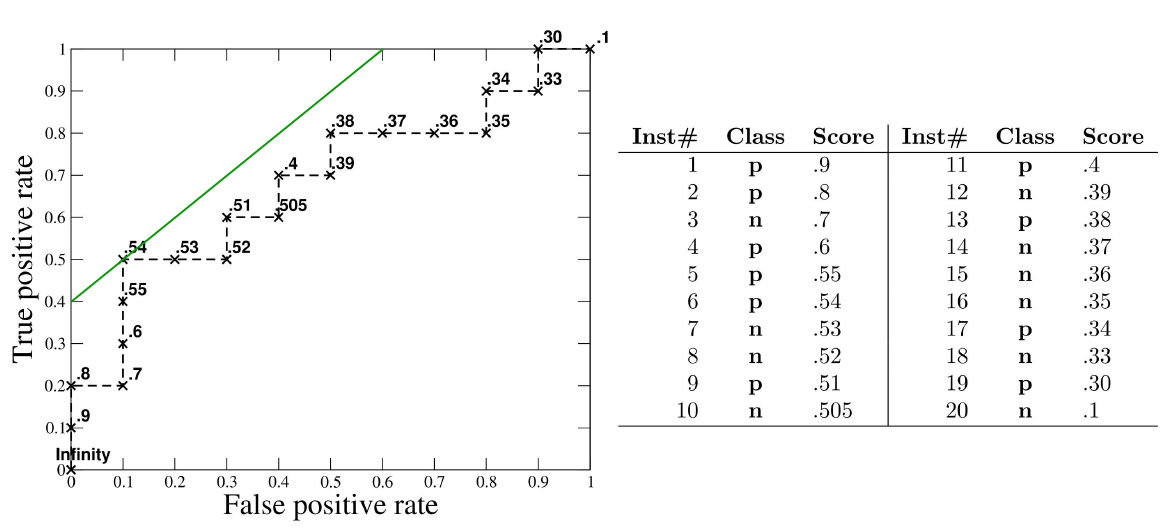
\includegraphics[scale=0.5]{Images/ROC2.png}
					\caption{Pour une instance de $p$, on monte,
							 et pour une instance de $n$, on va à droite}
					\label{fig:roc1}
				\end{figure}\noindent
				\begin{minipage}{0.45\textwidth}
					\vspace*{2cm}
					\begin{figure}[H]
						\centering
						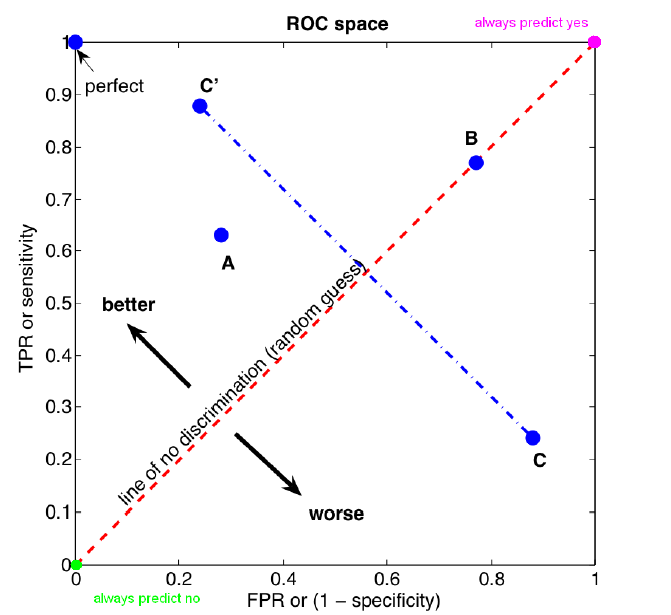
\includegraphics[scale=0.5]{Images/ROC.png}
						\caption{On prend la plus haute diagonale,
								 parallèle à la
								 ligne de discrimination, qui passe
								 par un des points}
						\label{fig:roc2}
					\end{figure}\noindent
				\end{minipage}\hfill
				\begin{minipage}{0.45\textwidth}
					\vspace*{-0.8cm}
					\begin{figure}[H]
						\centering
						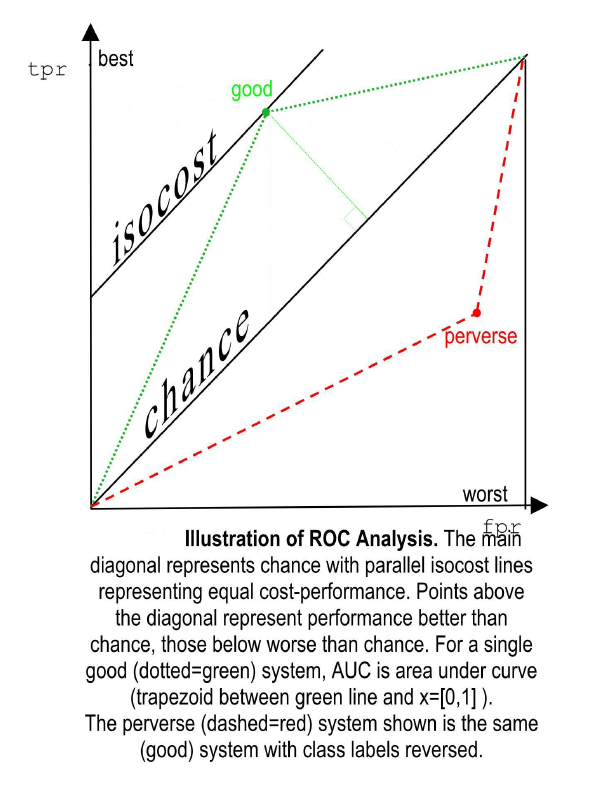
\includegraphics[scale=0.5]{Images/ROC3.png}
						\caption{Au plus la diagonale est haute,
								 au plus la classification est
								 bonne}
						\label{fig:roc3}
					\end{figure}\noindent
				\end{minipage}\noindent
				%
			%
			\subsubsection{Méthode \textit{Holdout}}
				\alinea Très semblable à l'usage de données de validation.
					On va \hl{diviser les données initiales en deux 
					ensembles de même taille. Un des ensemble qui sert 
					de données de test et l'autre de données d'entraînement}.
					\\
				%
				\alinea Les deux ensembles sont donc liés, il peut y avoir 
					un déséquilibre dans les labels. On pourrait donc
					avoir une classe moins représentée dans un ensemble,
					ce qui implique (si les classes sont bien réparties
					dans les données de base) que cette classe est représentée
					trop fort dans l'autre ensemble. Ceci peut impliquer
					un modèle biaisé de par le déséquilibre dans les données
					d'entraînement.
				%
			%
			\subsubsection{Random subsampling}
				\alinea Dans cette méthode, on va répéter la méthode
					\textit{holdout} $k$ fois, la découpe en deux ensemble
					étant aléatoire, chaque découpe sera différente.\\
				%
				\alinea On initialise un compteur $i$. Tant que $i < k$,
					on divise en deux les données, on améliore le modèle et
					on teste le modèle.\\
				%
				\alinea La précision du modèle obtenu est la suivante, 
					avec $acc_i$ la précision du modèle obtenu à 
					l'itération $i$.
					$$ \sum_{i=1}^{k} \frac{acc_i}{k} $$
				%
			%
			\subsubsection{Cross-validation}
				\alinea Cette fois-ci, \hl{chaque objet est utilisé le même
					nombre de fois pour entraîner le modèle, et une 
					seul et unique fois pour le tester.} Cette méthode
					se divise en deux techniques principales.
				%
				\subparagraph{k-fold} On divise les données initiales en
					$k$ sous-ensemble de même taille. \hl{On itère $k$ fois,
					et pour l'itération $i$, on choisit l'ensemble $i$
					comme ensemble de test et les $k-1$ autres comme 
					ensemble d'entraînement.}
				%
				\subparagraph{leave-one-out} Cas particulier du k-fold
					où $k = N$, $N$ étant le nombre d'objets présents dans
					les données. \hl{On a donc un seul objet par 
					sous-ensemble.}
					Cette approche utilise donc $N-1$ données d'entraînement
					à chaque itération (peu de chance d'\textit{underfitting})
					et un seul objet de test (si l'objet ne passe pas le test,
					le modèle sera considéré comme très mauvais). On a donc
					énormément de calculs à faire ($N$ modélisations) mais
					en moyenne le modèle résultant est bon (même si la 
					variance de la qualité du modèle est haute dû aux tests
					à un seul objet).
				%
			%
			\subsubsection{Bootstrap}
				\alinea Contrairement aux méthodes précédentes, les
					objets de cette méthode peuvent être réutilisés
					plusieurs fois pour entraîner le modèle. En effet, 
					la construction d'un extrait de \textit{bootstrap},
					qui sera utilisé comme ensemble d'entraînement se fait
					comme suit :
					\begin{enumerate}
						\setlength{\itemsep}{0pt}
						\setlength{\parskip}{0pt}
						\setlength{\parsep}{0pt}
						\item On tire au hasard un objet et on l'ajoute
							à l'extrait de \textit{bootstrap}.
						\item L'objet tiré est replacé afin qu'il puisse
							peut-être être de nouveau tiré dans une 
							prochaine itération.
						\item Recommencer jusqu'à obtenir un ensemble
							de taille voulue (paramètre).
					\end{enumerate}
					Une fois l'extrait construit, on l'utilise
					comme ensemble d'entraînement, les objets non présents
					dans l'extrait sont utilisés comme données
					de test. On itère $b$ fois, ce qui implique que $b$
					extraits de \textit{bootstrap} sont créés au cours de
					l'opération.\\
				%
				~\\
				%
				\alinea On estime que dans un extrait de taille $N$,
					$N$ étant le nombre d'objet dans le jeu de données de base,
					63,2\% des données de base y sont présent (et donc que
					36,8\% des données sont des doublons).\\
				%
				\alinea La précision d'un modèle construit peut se calculer 
					de plusieurs manières, la plus connue est le
					\textbf{.632 bootstrap}, définie comme suit avec
					$\epsilon_i$ la précision du modèle créé avec 
					l'extrait de \textit{bootstrap} de 
					l'itération $i$, et $acc_s$ la précision d'un modèle
					créé avec tous les objets des données de base en
					entraînement.
					$$ acc_{boot} = \frac{1}{b} \sum_{i=1}^{b}(0.632 
			   					    \cdot \epsilon_i + 0.368 \cdot acc_s) $$
				%
			%
		%
		\subsection{Méthode de comparaison de classificateurs}
		\alinea Pour comparer des résultats de classificateurs,
			surtout sur des jeux de test différents, il faut 
			passer par des tests statistiques. Par exemple,
			prenons deux modèles : $M_a$ et $M_b$. $M_a$ a une 
			meilleure précision que $M_b$, mais la précision de $M_a$
			a été calculé sur un jeu de test moins grand que celui de
			$M_b$. Il faut donc pouvoir mesurer la confiance que l'on
			peut accorder à la précision de $M_a$ par rapport à la
			grandeur de son ensemble de test.\\
		%
		~\\
		%
		\alinea Pour connaître l'intervalle de confiance, 
			il faut déterminer la distribution de probabilité
			qui domine la mesure de précision. Pour ce faire,
			on peut modéliser le problème de classification en
			une expérience binomiale:
			\begin{enumerate}
				\setlength{\itemsep}{0pt}
				\setlength{\parskip}{0pt}
				\setlength{\parsep}{0pt}
				\item Expérience de $N$ essais indépendants 
					donnant soit un \myul{succès}, 
					soit un \myul{échec}.
				\item La probabilité $p$ d'obtenir un succès à chaque
					essai est constante.
			\end{enumerate}
		%
		\newpage
		%
			Soit $X$ le nombre de succès sur $N$ essais, la 
			probabilité d'en avoir $v$ est la suivante:
			$$ P(X=v) = \binom{N}{v} p^v (1 - p)^{N-v} $$
		%				
		\alinea \hl{Pour la classification, $p$ est la vrai précision
			du modèle, $X$ est le nombre d'instances bien classifiées,
			$N$ le nombre total d'objets.} Si on prends la précision
			empirique, normalisée par rapport à la taille du jeu
			de données de test, \hl{$\frac{X}{N}$} (moyenne = $p$, 
			variance = $\frac{p(1 - p)}{N}$), c'est aussi une 
			distribution normale. Son intervalle de confiance est
			souvent approximé par une distribution normale pour
			$N$ suffisamment grand : 
			$$ P \left( -Z_{\alpha/2} \leq \frac{acc - p}%
				{\sqrt{p(i-p)/N}} \leq Z_{1-\alpha/2} \right) 
						= 1 - \alpha $$
			Avec $-Z_{\alpha/2}$ et $Z_{1-\alpha/2}$ les bords
			supérieurs et inférieurs
			obtenus par distribution normale avec une confiance de 
			$1-\alpha$.\\
		%
		~\\
		%
		\alinea Les formules suivantes permettent alors de conclure
			sur la différence entre les précisions comparées/
			$$ I (= d_t) = d \pm z_{\alpha/2} \cdot 
				\hat{\sigma} = \mathbf{[} d - z_{\alpha/2} \cdot 
				\hat{\sigma}\mathbf{,}\ \ d + z_{\alpha/2} \cdot 
				\hat{\sigma}\mathbf{]} $$
			$$ d = e - f $$
			$$ 1-\alpha = 90\%\ (Certitude) \Leftrightarrow 
				\alpha = 10\% $$
			$$ z_{\alpha/2} = 1.65\ (Confiance) $$
			$$ \hat{\sigma} = \sqrt{\dfrac{e(1 - e)}{n} + 
				\dfrac{f(1 - f)}{m}} $$
			Avec $e$ (\textit{resp.} $f$) représente le 
			pourcentage d'instances mal classifiées
			dans le modèle 1 (\textit{resp.} 2) et $n$ 
			(\textit{resp.} $m$) représente le nombre total
			d'instances classées par le modèle 1 (\textit{resp.} 2).\\
		%
		\alinea Les précisions des deux modèles sont alors 
			considérées comme significativement différentes si
			0 n'est pas couvert par I. \\
			%
		%
		~\\
		%
		\myul{\textbf{\hl{Remarque}}} -- On peut aussi utilise l'intervalle
			de confiance pour évaluer un élagage d'arbre. Comme le montre
			la figure \ref{fig:pruning}. On y voit qu'on regarde à élaguer
			le noeud qui a été divisé selon l'attribut "health plan
			contribution". On calcule alors l'intervalle de confiance 
			pour chacun des fils de ce noeud, en prenant en compte la 
			précision du fils concernant la classe "bad".\\
			On a donc $n$ le nombre d'objet total, $X$ le nombre d'objet
			libellé "bad", et $p_1$ et $p_2$ les bornes, inférieure et 
			supérieures, de l'intervalle de confiance.
		%
		\begin{figure}[H]
			\centering
			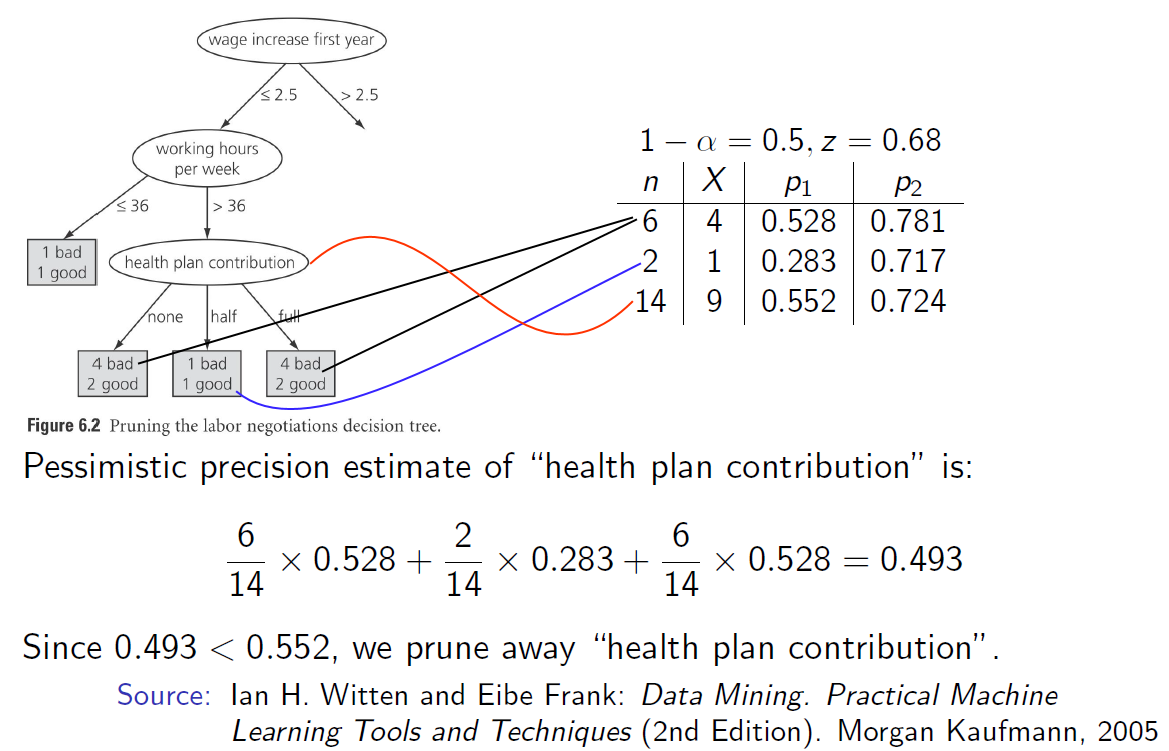
\includegraphics[scale=0.45]{Images/pruning.png}
			\caption{L'élagage est dans ce cas utile devrait être fait,}
					 car le split n'apporte pas d'informations utiles.
			\label{fig:pruning}
		\end{figure}\noindent
		%
		\alinea On compare donc ensuite la somme pondérée de la borne 
			inférieure des fils (estimation \myul{pessimiste}) avec
			la borne inférieur du parent. Si cette dernière est 
			plus élevée (comme dans l'exemple), cela veut dire que
			la division n'était pas utile et fait perdre en confiance, 
			on peut donc élaguer.
		%
	%
	\newpage
	%
	\section{Types d'algorithmes}
		\alinea Il existe plusieurs type d'algorithmes construisant des 
			modèles de classification. En voici quelques-uns.
		%
		\subsection{Nearest Neighbours (kNN, Lazy)}
			\alinea Cette technique s'appuie sur la notion de distance
				entre les instances. Plusieurs distances peuvent être
				considérées (Euclidienne, Manhattan, ...). Voici quelques
				définitions de \hl{distances} en fonction des 
				types d'attributs.
				\begin{itemize}
					\setlength{\itemsep}{0pt}
					\setlength{\parskip}{0pt}
					\setlength{\parsep}{0pt}
					\item \myul{Un attribut numérique uniquement} : différence.
					\item \myul{Plusieurs attributs numériques} : normalisation
						des valeurs + distance Euclidienne, ou Manhattan.
					\item \myul{Attributs nominaux} : 0 si valeur identique,
						1 sinon.
				\end{itemize}
			%
			\alinea Il reste ensuite à regrouper les objets en groupe en 
				fonction de la distance qu'il y a entre chaque objets
				et leur $k$ plus proches voisins.
			%
		%
		\subsection{Règles de classification}
			\alinea Classificateur qui consiste en une série de $k$ 
				règles, liées entre-elles par des "ET".\\				
			%
			\alinea Exemple :
				\begin{center}
					Si $a < 5$ et $b < 4$ : classe = oui\\
					Si $a > 2$ et $c > 3$ : classe = non\\
					Si $b > 3$ et $d > 2$ : classe = oui\\
					...
				\end{center}
			%
			\alinea Pour le classificateur \hl{\texttt{OneR}}, le but est
				de tester pleins de règles concernant chacune un seul
				attribut, chaque règle testées prenant les meilleurs
				valeurs "limites" de l'attribut pour classifier, et seule
				la meilleure règle est gardée.\\
			%
			~\\
			%
			\alinea Pour \hl{\texttt{Prism}} par contre, on se concentre 
				sur les classes. Prenons comme exemple la figure 
				\ref{fig:prism} comme exemple. Dans cet exemple, il y 
				a deux classes : "oui", et "non", avec 5 objets dans 
				chaque classe. On va ici s'intéresser 
				à classer "non" au mieux. On va donc énumérer des
				règles simples (cf. figure \ref{fig:prism}), et 
				regarder la précision de classification des instances
				correspondant à ces conditions.
			%
			\begin{figure}[H]
				\centering
				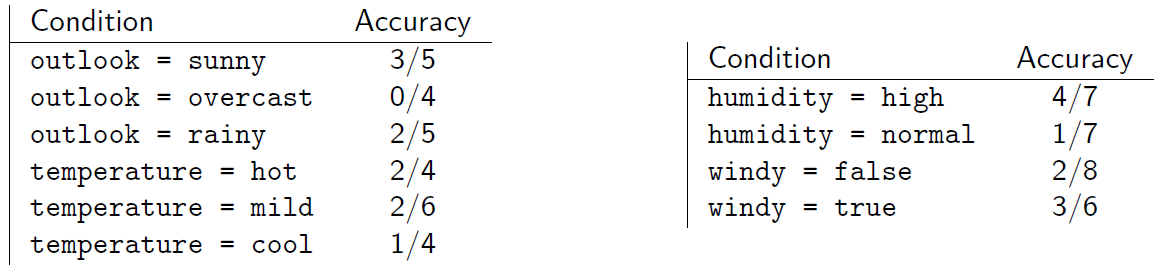
\includegraphics[scale=0.4]{Images/prism.png}
				\caption{Règle et précision de classification pour la classe
						 "non"}
				\label{fig:prism}
			\end{figure}\noindent
			%
			\alinea La précision la plus élevée est 3/5. Nous choisissons
				donc la condition \texttt{outlook = sunny}. On va ensuite 
				regarder s'il faut continuer à chercher des règles ou pas.
				La figure \ref{fig:prism2} montre les 5 instances
				correspondant à la condition \texttt{outlook = sunny}
				que l'on vient de choisir.
			%
			\begin{figure}[H]
				\centering
				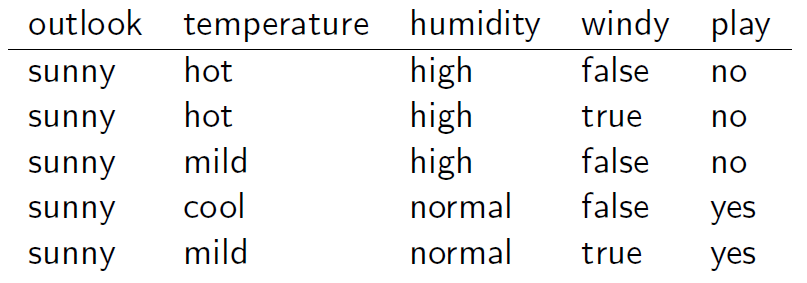
\includegraphics[scale=0.4]{Images/prism2.png}
				\caption{On peut encore raffiner la condition en
						 rajouter des conditions}
				\label{fig:prism2}
			\end{figure}\noindent
			%
			\alinea Si on recommence à regarder pour quelle règle 
				on classe le mieux les "non" pour les cinq instances
				restantes, on obtient le tableau de la figure \ref{fig:prism3}.
			%
			\begin{figure}[H]
				\centering
				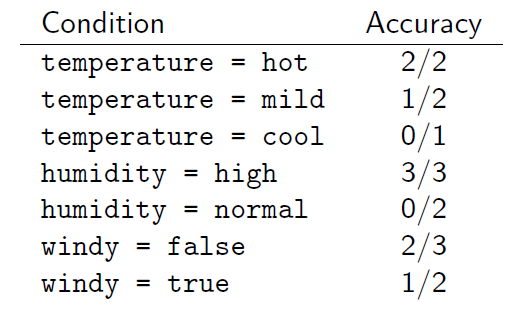
\includegraphics[scale=0.5]{Images/prism3.png}
				\caption{L'égalité entre deux règles se brise par le
						 le nombre d'instances couvertes}
				\label{fig:prism3}
			\end{figure}\noindent
			\alinea On remarque une égalité entre \texttt{temperature = hot}
				et \texttt{humidity = high}. Nous prendrons la deuxième 
				condition car c'est elle des deux qui couvre le plus d'objets.
				Seulement, la règle entière \texttt{si outlook = sunny et
				humidity = high} ne couvre que 3 ces 5 instances "non".
				On recommence depuis le début, mais cette fois-ci en
				retirant les objets répondant à la règle déjà trouvée,
				etc... jusqu'à obtenir le maximum d'instances "non" bien 
				classées. Puis, on peut recommencer le travail avec les
				classes "yes".\\
			%
			~\\
			%
			\myul{\hl{\textbf{Remarque}}} -- Les règles trouvées par
				\texttt{Prism} sont \textit{sound} mais pas 
				\textit{complete}. En effet, on est sur que \myul{les 
				règles sont vraies pour le jeu de données} d'entraînement
				(\textit{sound}) mais elles ne sont \myul{pas vraies pour 
				n'importe quel jeu de données} (non \textit{complete})
			%
		%
		\newpage
		%
		\subsection{Arbres IBk}
			\alinea Arbres de décisions avec des règles sur les attributs.
				On peut noter que ces arbres sont parfois trop complexes
				pour rien (problème du sous arbres dupliqué), et que 
				les règles s'y trouvant ne sont pas garantie \textit{sound}
				ni \textit{complete}. \\
			%
			~\\
			%
			\alinea On peut noter qu'il y a deux types de règles de manière 
				générale (pas que pour les arbres). Ceux-ci sont expliqués
				sur la figure \ref{fig:ibk}.
			%
			\begin{figure}[H]
				\centering
				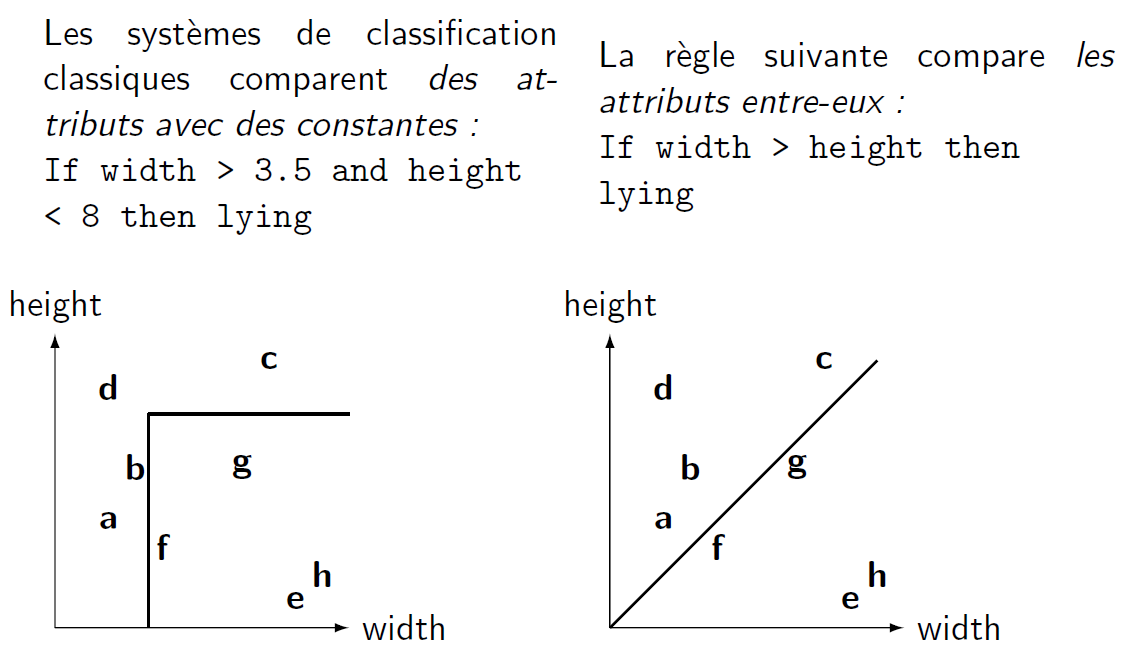
\includegraphics[scale=0.3]{Images/ibk.png}
				\caption{Il y a deux types de règles}
				\label{fig:ibk}
			\end{figure}\noindent
			%
		%
		\subsection{Naive Bayes}
			\alinea	Ce classificateur utilise la règle de Bayes. C'est une 
				règle de probabilité qui dit : 
				$$ Pr(H | E) = \frac{Pr(E | H) \cdot Pr(H)}{Pr(E)} $$
				Avec $Pr(x | y)$ voulant dire la probabilité de $x$, sachant
				que $y$.\\
			%
			~\\
			%
			\alinea Pour classifier, on utilisera cette règle afin de 
				trouver la probabilité pour l'objet $k$ 
				d'appartenir à une classe $i$, en
				sachant les attributs de cet objet 
				(=$\text{Pr}(Class_i | Attributes_k)$). Normalement, 
				un tel calcul
				est très couteux et parfois infaisable quand on a pas
				toutes les informations, car :
				$$ \text{Pr}(Class_i | Attributes_k) = 
				    \frac{\text{Pr}(Att_{1_k}\& 
					Att_{2_k} \& \ldots \& Att_{j_k}| Class_i) 
					\cdot \text{Pr}(Class_i)}{\text{Pr}(Attributes_k)} $$
				Mais on admet une certaine naïveté, en pensant que tous
				les attributs sont indépendants l'un de l'autre, et donc
				que :
				$$ \text{Pr}(Class_i | Attributes_k) =  \frac{
						\text{Pr}(Att_{1_k} | Class_i) \cdot
						\text{Pr}(Att_{2_k} | Class_i) \cdot
						\ldots \cdot
						\text{Pr}(Att_{j_k} | Class_i) \cdot
						\text{Pr}(Class_i)}{\text{Pr}(Attributes_k)}$$
				Avec $Att_{l_k}$ l'attribut $l$ de l'objet $k$.	
			%
		%
	%
%
\part{Analyse par association}
	\alinea Le but de ce chapitre est de développer des techniques
		permettant de déduire des liens entre des entrées de jeu 
		de données. Un exemple répandu est celui du panier d'achat 
		d'un client de magasin, on pourrait trouver des liens entre
		l'achat de certaines marchandises avec l'achat d'autres. On 
		appel ces liens des \textbf{règles d'association}. Exemple :
		$$\{Langes\} \longrightarrow \{Bieres\}$$
		Ce qui impliquerait qu'il y a une forte corrélation entre
		la vente de langes et la vente de bières, ce qui veut dire
		que les gens qui achètent des langes ont de grandes chance d'acheter
		de la bière en même temps.
	%
	\paragraph{\point Domaines d'application}~\\~\\
		\alinea \hl{En plus de ces paniers de marchandises, on trouve l'utilité
			dans la bio-informatique, les diagnostiques médicaux, 
			le Web mining et l'analyse de données scientifiques. Par exemple,
			en géologie, des modèles d'associations peuvent révéler 
			d'intéressantes relations entre les océan, les continents, et 
			les processus atmosphériques.}
		%
	%
	\paragraph{\point Définition du problème}~\\~\\
		\alinea Nous allons définir ci dessous les différents
			termes et hypothèses que nous utiliserons.
		%
		\subparagraph{Représentation binaire} Les jeux de données
			traitées seront supposé représentable de manière binaire.
			Dans l'exemple du panier d'achat, on aura une variable par
			type de produit, cette variable vaudra 1 si l'objet a été acheté,
			et 0 sinon. \hl{Nous pouvons noter que dans ce cas, la variable
			est asymétrique de par le fait que si la variable est à 0,
			elle ne sera pas utilisée, en effet, il n'est pas très utile 
			de savoir que nous n'avons pas acheté un certain objet ...}.
		%
		\subparagraph{\textit{Itemsets}} Soit
			$I = \{i_1, i_2, \ldots, i_d\}$ être l'ensemble de tous 
			les objets (\textit{itemset}) considérés et 
			$T = \{t_1, t_2, \ldots, t_N\}$ être l'ensemble des transactions
			effectuées. Chaque transaction de $t_i$ est un sous-ensemble
			de $I$. Si un \textit{itemset} comporte $k$ objets, il est 
			appelé \textit{$k$-itemset}. L'\textit{itemset} vide est accepté.
		%
		\subparagraph{\textit{Support Count}} Soir la largeur de la 
			transaction (\textit{transaction width} $= |t_i|$) étant le nombre
			d'objets présent dans la transaction. Le \textit{support count}
			($\sigma(X)$) est défini comme suit : 
			$$ \sigma(X) = |\left\lbrace t_i | X \subseteq t_i,\ \ t_i \in T
				\right\rbrace| $$
			On a donc le nombre de transactions dans $T$ dans lesquels
			apparaît l'ensemble $X$ d'objets.
		%	
		\subparagraph{Règles d'association} Implication écrite sous la forme
			$X \longrightarrow Y$ dans laquelle $X$ et $Y$ sont disjoints
			($X \cap Y = \emptyset$). La solidité d'une règle est
			mesurée en terme de son \textit{Support} et de sa
			\textit{Confidence}. Soit $N$ le nombre total de transaction
			($ = |T|$), on a 
			\begin{align*}
				\text{Support},\ \ s(X \longrightarrow Y) &= 
							\frac{\sigma(X \cup Y)}{N}\\
				\text{Confidence},\ \ c(X \longrightarrow Y) &= 
							\frac{\sigma(X \cup Y)}{\sigma(X)}
			\end{align*}
			On peut noter qu'une règle ayant un faible \textit{Support}
				peut être dû à la chance, et que la \textit{Confidence}
				défini la confiance que l'on peut avoir dans la règle.
			\hl{La \textit{Confidence} donne aussi une estimation
			de $\text{Pr}(Y | X)$}. De plus, \hl{le \textit{support} d'une
			règle $X \longrightarrow Y$ ne dépend que de l'ensemble
			$X \cup Y$}. Donc, les six règles suivantes ont le
			même \textit{support} :
			\begin{figure}[H]
				\centering
				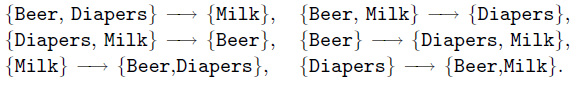
\includegraphics[scale=0.725]{Images/support}
			\end{figure}\noindent
			%
			\hl{Il faut noter que l'inférence faite par une règle 
			d'association ne donne pas de causalité}.
			L'achat des langes n'est pas la cause de l'achat de bières.
		%
	%
	\section{Découverte de règles}
		%
		\begin{tabular}{lp{10.25cm}}
			\myul{\textbf{Découverte de règles d'association}} & 
			\red{\'Etant donné un ensemble de transaction $T$, trouver toutes
			les règles règles ayant un \textit{support} $ \geq minsup$ et
			une \textit{confidence} $ \geq minconf $, où $minsup$ et 
			$minconf$ sont deux seuils à définir.}
		\end{tabular}\noindent~\\\noindent~\\\noindent%
		%
		\alinea Un ensemble de transaction
			qui contient $d$ objets peut générer $R$ règles au total.
		%
		$$ R = 3^d - 2^{d+1} + 1 $$
		%		
		\alinea \myul{\hl{On peut le prouver}} de la manière suivante. 
			Soit le tableau $\left[L, R, L, X, X, ..., X\right]$ 
			représentant une règle. Les indices du tableau sont les 
			différents objets, $L$ veut dire "l'objet se trouve dans
			la partie gauche de la règle", $R$ veut dire "l'objet se trouve
			dans la partie droite de la règle"
			et $X$ veut dire "ne fait pas partie de la règle". Le tableau
			donné donnerait donc la règle $\{obj_0, obj_2\} \longrightarrow
			\{obj_1\}$.\\
		%
		\alinea On a donc 3 possibilités par case, donc $3^d$. Mais on ne
			peut pas avoir que des $X$ et des $R$, 
			ni que des $X$ et des $L$, on doit donc retirer des $3^d$ 
			possibilité 2 fois $2^d$ ($X$ et $L$ ou $X$ et $R$ = 2 
			possibilités par case), et $2\cdot 2^d = 2^{d+1}$. Et enfin,
			on se rend compte que dans ce qu'on a retiré, il y avait
			deux fois l'ensemble de contenant que des $X$, on doit 
			donc rajouter $1$ pour compenser. On a donc bien 
			$3^d - 2^{d+1} + 1$.\\
		%
		\newpage\noindent
		%
		\alinea On peut conclure qu'il est impossible de toutes les générer
			par force brute, il faut donc trouver des astuces pour générer
			de bonnes règles en un temps raisonnable. On a donc deux tâches
			principales à remplir :\\~\\
			\begin{tabular}{lp{10cm}}
				(1) \myul{\textbf{Génération de \textit{Frequent
					Itemsets}}} &
					\red{Trouver tous les itemsets dont le \textit{support}
					satisfait $minsup$.}\\
				(2) \myul{\textbf{Génération de règle}} &
					\red{Extraire les 
					règles à haute \textit{confidence}, qui seront 
					appelées les règles "fortes".} Généralement moins 
					couteux que (1).
			\end{tabular}
		%
	%
	\section{Génération de \textit{frequent itemsets}}
		\alinea \hl{Un ensemble de $k$ objets peut potentiellement générer
			$2^k - 1$ itemsets fréquents}, étant donné que dans un
			itemset candidat, un objet peut soit être présent, soit ne
			pas l'être. Un algorithme de force brute devrait donc effectuer
			$O((2^k - 1)Nw)$ opérations pour calculer les \textit{support} de 
			tous les itemsets possibles, car il faut comparer les itemsets
			possibles avec les $N$ transaction qui ont une largeur de 
			maximum $w$. Il y a deux manières de réduire le nombre de 
			calculs.
		%
		\begin{enumerate}
			\setlength{\itemsep}{0pt}
			\setlength{\parskip}{0pt}
			\setlength{\parsep}{0pt}
			\item \hl{Réduire le nombre d'itemset à comparer} (cf. la section
				\ref{sec:rules:apriori}).
			\item \hl{Réduire le nombre de comparaisons en utilisant des
				structures de données avancées.}
		\end{enumerate}
		%
		\subsection{Le principe \textit{Apriori}}\label{sec:rules:apriori}
			\alinea Ce principe permet de réduire le nombre d'itemsets à
				comparer aux transactions. Ce principe dit qu'un itemset
				fréquent ne contient que des sous-ensembles fréquents.
				Et donc, ce qui nous intéresse, que\hl{ si un itemset est 
				non-fréquent, tous ses super-ensembles sont non-fréquents}.\\
			%
			~\\
			%
			\alinea Ceci est rendu possible grâce à l'anti-monotonicité
				de la mesure \textit{support}.\\~\\
			%
			\begin{tabular}{lp{10cm}}
				\myul{\textbf{Propriété de Monotonicité}} &
					\red{Soit $I$ un ensemble d'objets, et $J = 2^I$ l'ensemble 
					des parties de I. Une mesure $f$ est monotone
					(ou bornée supérieurement) si:
					$$ \forall X, Y \in J : (X \subseteq Y) 
							\Longrightarrow f(X) \leq f(Y) $$}		
			\end{tabular}~\\~\\
			Par analogie, une propriété $f$ est anti-monotone si:
				$$ \forall X, Y \in J : (X \subseteq Y) 
							\Longrightarrow f(X) \geq f(Y) $$
			%
			Le principe \textit{Apriori} peut être appliqué à n'importe 
			quelle mesure anti-monotone incorporée à l'algorithme.
		%
		\subsection{Génération d'itemsets fréquents avec \textit{Apriori}}
			\alinea La figure \ref{fig:apriori:gen} illustre la génération
				d'éléments.
			%
			\begin{figure}[H]
				\centering
				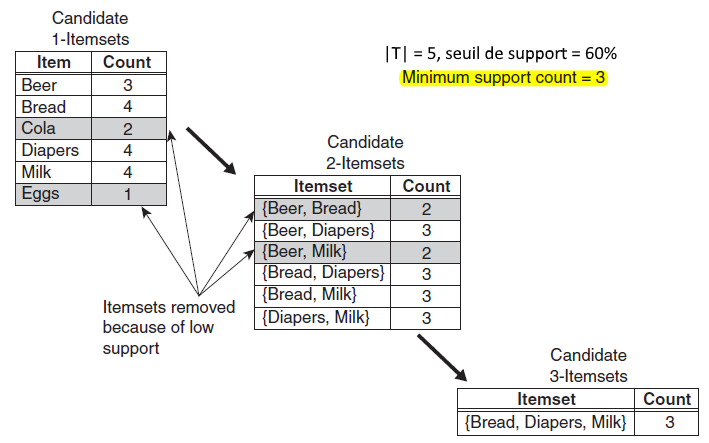
\includegraphics[scale=0.75]{Images/apriori_gen.png}
				\caption{}
				\label{fig:apriori:gen}
			\end{figure}\noindent
			%
			\begin{figure}[H]
				\centering
				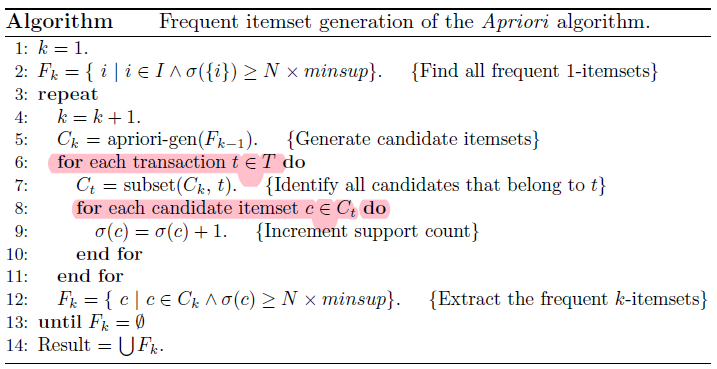
\includegraphics[scale=0.75]{Images/apriori_algo.png}
				\caption{L'algorithme permettant d'extraire les itemsets
						 fréquents}
				\label{fig:apriori:algo}
			\end{figure}\noindent
			%
			L'implémentation de la fonction \texttt{apriori-gen} est
				couvert dans la partie \ref{sec:apriori:gen} et la 
				fonction \texttt{subset} est expliquée dans la section
				\ref{sec:apriori:count}. L'algorithme prend $k_{max} +1$
				itération, où $k_{max}$ est la taille du plus grand
				itemset fréquent.
			%
		%
		\subsection{Génération de candidats et élagage}\label{sec:apriori:gen}
			\alinea La fonction \texttt{apriori-gen} de l'algorithme Apriori
				génère des candidats suivants deux opérations:\\~\\
				\begin{tabular}{lp{12cm}}
					(1) \myul{\textbf{\hl{Génération de candidat}}} & 
						\red{Génère des candidats de taille $k$ à partir 
							des itemsets fréquents de taille $k-1$ déjà générés.}\\
					(2) \myul{\textbf{\hl{\'Elagage des candidats}}} & 
						\red{Supprime les candidats n'ayant pas assez de
						\textit{support}.}
				\end{tabular}~\\~\\
			%
			\alinea L'étape (2) doit en fait regarder tous les itemsets de
				taille $k$ générés n (1), et supprimer ceux qui contiennent
				des sous-itemsets (pas besoin de regarder ceux de taille 1)
				non-fréquents, par le principe d'\textit{Apriori}. C\hl{eci
				représente $O(k)$ opérations pour chaque itemset de
				taille $k$}, cependant, ce nombre sera réduit plus tard.\\
			%
			~\\
			%
			\alinea Une bonne méthode pour générer des itemsets candidats doit
				suivre les directives suivantes:
				\begin{enumerate}
					\setlength{\itemsep}{0pt}
					\setlength{\parskip}{0pt}
					\setlength{\parsep}{0pt}
					\item[(a)] \hl{Elle devrait éviter de générer trop de 
						candidats inutiles (avec sous-ensemble non-fréquent).}
					\item[(b)] \hl{Elle doit être certaine de ne pas retirer
						de candidats valides}
					\item[(c)] \hl{Elle ne devrait pas générer plus d'une fois
						le même candidat.} En effet, il est possible de
						créer $\{a,b,c\}$ en fusionnant $\{a, b\}$ et $\{c\}$
						mais aussi en fusionnant $\{a, c\}$ et $\{b\}$, il
						faut donc éviter les doublons.
				\end{enumerate}
			%
			\subsubsection{Force brute}
				\alinea Le principe est de considérer tous les itemsets
					de taille $k$ comme candidat potentiel. On a donc
					$\binom{d}{k}$ itemsets générés à chaque étape,
					et vu que $O(k)$ opérations doivent être effectuées par
					itemset, il y a $O(d\cdot 2^{d-1})$ opérations.
				%
			%
			\subsubsection{$\mathbf{F_{k-1} \times F_1}$}
				\alinea une autre méthode de génération est de 
					créer des itemsets de taille $k$ en prenant 
					les itemsets fréquents de taille $k-1$ et d'y rajouter 
					un par un les objets fréquents (itemset de taille 1).\\
				%				
				\alinea La méthode respecte (b), mais pas (c). Une manière de 
					respecter (c) serait de \hl{s'assurer de respecter l'ordre
					lexicographique} lors de la création de nouveaux 
					itemsets. \\
				%
				\textbf{Exemple} : $\{a, b\}$ peut être 
					augmenté
					avec $\{c\}$ pour former  $\{a,b,c\}$, mais pas 
					$\{a, c\}$ et $\{b\}$ car $b$ vient se rajouter
					après $c$, qui est plus grand d'un point de vue
					lexicographique.\\
				%
				\alinea La méthode génère cependant pas mal d'itemsets
					inutiles. En effet, admettons que l'on sache que 
					$\{a,c\}$ est non-fréquent, la méthode va tout
					de même créer $\{a,b,c\}$ en fusionnant $\{a,b\}$
					et $\{c\}$.
				%
			%
			\newpage
			%
			\subsubsection{\hl{$\mathbf{F_{k-1} \times F_{k-1}}$}}
				\alinea \hl{C'est la méthode utilisée en pratique}, 
					elle consiste à fusionner deux itemsets fréquents de taille
					$k-1$ qui ont chacun $k-2$ éléments en commun, tout
					en \hl{gardant l'ordre lexicographique discuté au point
					précédent}.\\
				\textbf{Exemple :} on fusionnerait $\{a,b,c\}$ avec
					$\{a,b,d\}$ pour obtenir $\{a,b,c,d\}$ car ils ont $a$ et
					$b$ en commun. \hl{Mais pour ce faire, il faut bien
					vérifier que le sous-ensemble commun de taille $k-2$ 
					est fréquent.}
				%
			%
		%
		\subsection{Compter le \textit{support count}}\label{sec:apriori:count}
			\alinea Le principe de cette étape est de compter dans combien de
				transaction se retrouve un itemset candidat. Les étapes
				d'avant vont générer un ensemble itemsets de taille fixe $k$.
				\hl{On va donc préférer énumérer tous les sous-ensemble 
				de taille
				$k$ contenu dans chaque transaction et incrémenter les
				itemsets s'y retrouvant}. Ce faisant, on ne va
				parcourir qu'une seul fois toutes les transactions.
				La figure \ref{fig:support:count} illustre la technique 
				utilisée.
			%
			\begin{figure}[H]
				\centering
				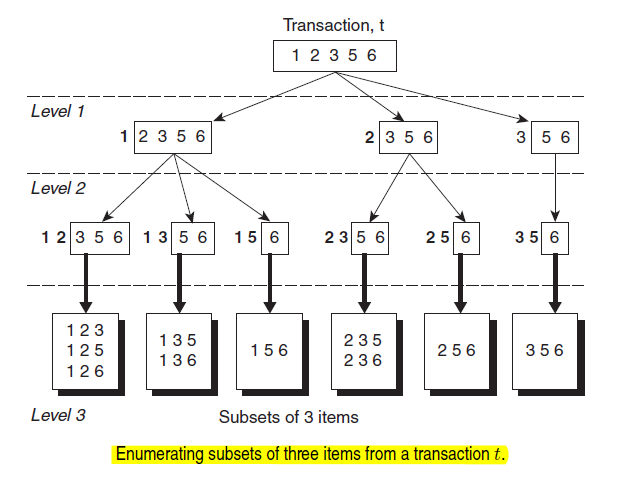
\includegraphics[scale=0.75]{Images/support_count}
				\caption{Chaque noeud du niveau $j$ va se fixer un préfixe
						 qui lui est propre de taille $j$}
				\label{fig:support:count}
			\end{figure}\noindent
			%
			Il reste alors à retrouver les itemsets candidats à incrémenter.
			Une méthode pour faire ça est de \hl{"pousser"} les sous-ensemble
			générés par l'énumération (e.g. ensembles de taille 3 de la 
			figure \ref{fig:support:count}) \hl{dans un arbre de hachage}
			Dans lequel les candidats sont divisés selon une table de hachage..
			Ceci est illustré sur la figure \ref{fig:support:tree}.
			%		
			\begin{figure}[H]
				\centering
				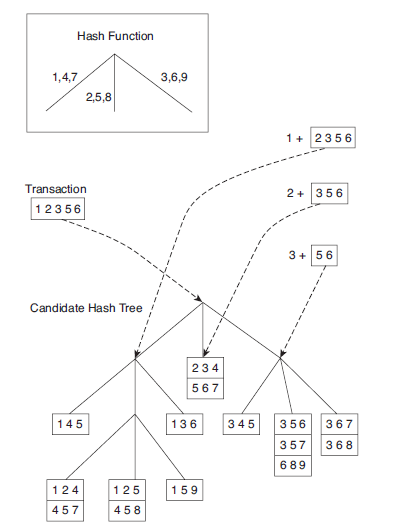
\includegraphics[scale=0.7]{Images/support_tree}
				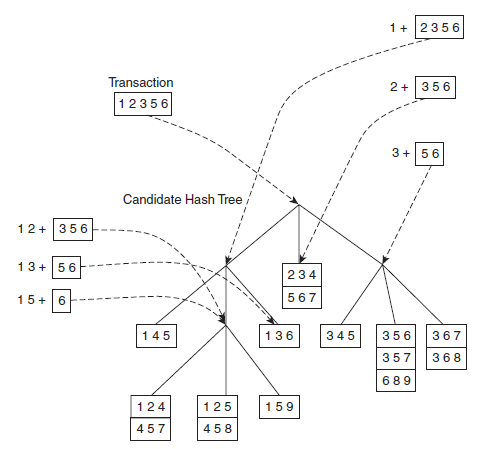
\includegraphics[scale=0.7]{Images/support_tree2}
				\caption{Dés lors, pas besoin de comparer tous les candidats,}
						 mais juste ceux présents dans la partie de l'arbre\\
						 où le sous-ensemble a été "poussé"
				\label{fig:support:tree}
			\end{figure}\noindent
			%
			\begin{figure}[H]
				\centering
				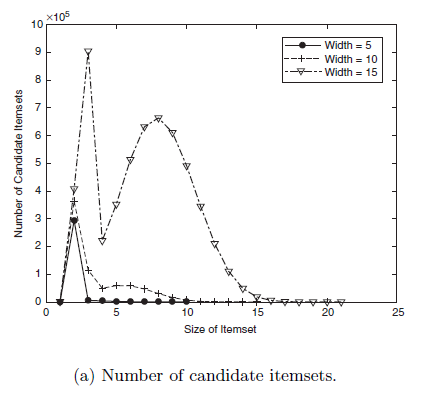
\includegraphics[scale=0.75]{Images/freq_it_a}
				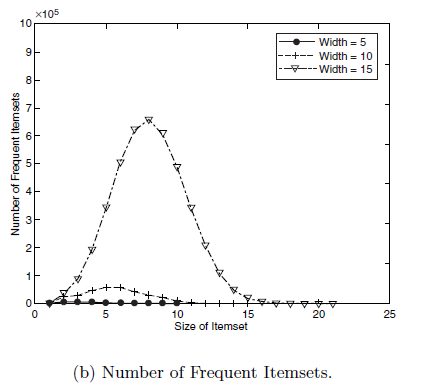
\includegraphics[scale=0.75]{Images/freq_it_b}
				\caption{Si la largeur moyenne d'une transaction}
						 est de 10, \hl{les itemsets fréquents de taille}\\
						 \hl{bien plus grande que 10 sont peu probables}
				\label{fig:freq_it:a}
			\end{figure}\noindent
			%
			\begin{figure}[H]
				\centering
				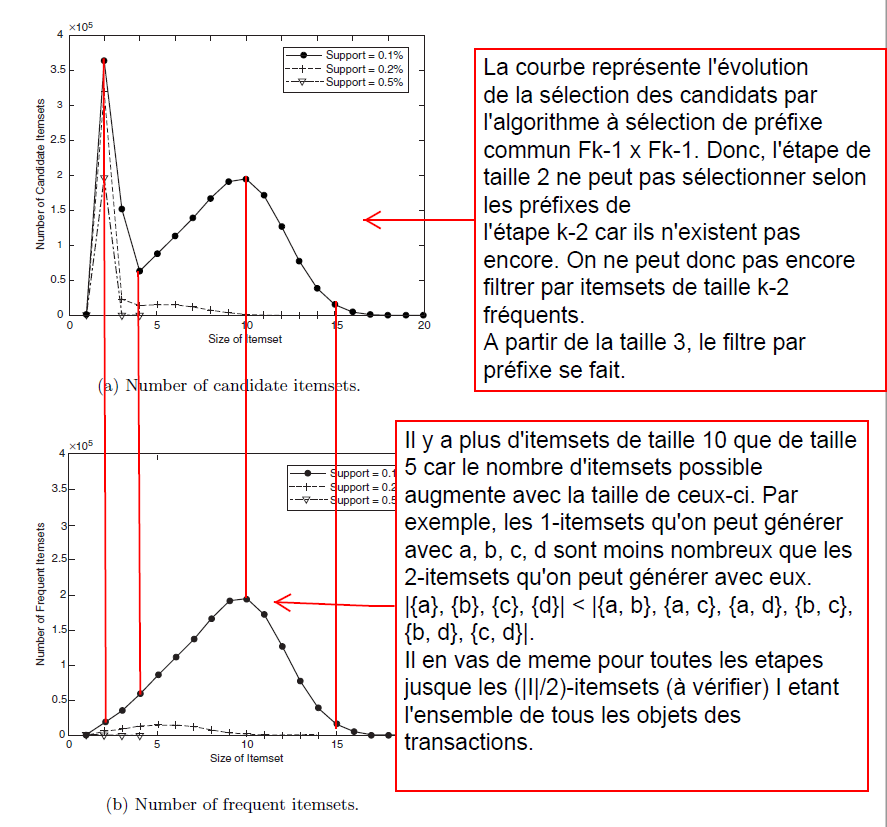
\includegraphics[scale=0.75]{Images/support_treshold}
				\caption{\hl{Important}}
				\label{fig:support_threshold}
			\end{figure}\noindent
			%
		% La section sur la complexité est passée car le prof a insisté
		% sur le fait ques c'était pas important...
	%
	\newpage
	%
	\section{Génération de règles d'associations}
		\alinea Cette partie est moins importante à optimiser car \hl{on
			a plus besoin d'accéder à la base de donnée}, ce qui prenait
			du temps. En effet, on connaît, les itemsets fréquents, grâce 
			à l'étape précédente, et pour calculer la \textit{confidence},
			on a juste besoin du support count des règles, ce qui est 
			déjà calculé.\\
		%
		~\\
		%
		\alinea Chaque itemset candidat $Y$ peut générer $2^k - 2$ 
			règle. \myul{\textbf{\hl{On peut le prouver}}}. En effet,
			Chaque objets d'$Y$ doit se retrouver dans la règle, chaque
			objet peut donc être soit à gauche, soit à droite de la règle.
			on a donc $2^k$ possibilités de combinaisons, mais on ne 
			doit pas considérer les règle $\{\} 
			\longrightarrow Y$ et $Y \longrightarrow \{\}$, on doit
			donc en retirer 2.\\
		%
		\alinea On peut donc générer des règles avec $Y$ en découpant 
			$Y$ en deux sous-ensembles : $X$ et $Y\setminus X$ afin de
			créer la règle $X \longrightarrow Y \setminus X$.
		%
		\subsection{\'Elagage basé sur la \textit{confidence}}
			\alinea On ne peut plus se baser sur le principe 	
				d'\textit{Apriori}, car la mesure de \textit{confidence} 
				n'est pas anti-monotone. Néanmoins, en comparant les règles 
				générées par le même itemset fréquent $Y$, \hl{le théorème
				suivant	s'applique}:
				\begin{align*}
				   &\text{\textbf{Si}}\ &\text{une règle } X\longrightarrow Y
				   			\setminus X 
					\text{ ne satisfait pas le seuil } minconf, \\
					&\text{\textbf{Alors}},\ &\forall X' \subseteq X, 
					  X' \longrightarrow Y \setminus X' \text{ ne 
					  satisfait pas non plus le seuil } minconf
				\end{align*}
			%
		%
		\subsection{Génération de règle dans l'algorithme Apriori}
			\alinea L'idée est de fusionner les parties droites de
				règles avec une \textit{confidence} élevée pour en former
				des nouvelles, qui seront elles-mêmes de confiance de par
				le théorème précédent.
			%		
			\begin{figure}[H]
				\centering
				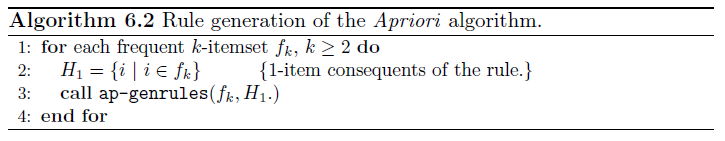
\includegraphics[scale=0.75]{Images/conf_algo1}
				\caption{Génération de règles à partir de tous}
				les itemsets fréquents générés à l'étape précédente.
				\label{fig:conf:algo1}
			\end{figure}\noindent
			%
			\begin{figure}[H]
				\centering
				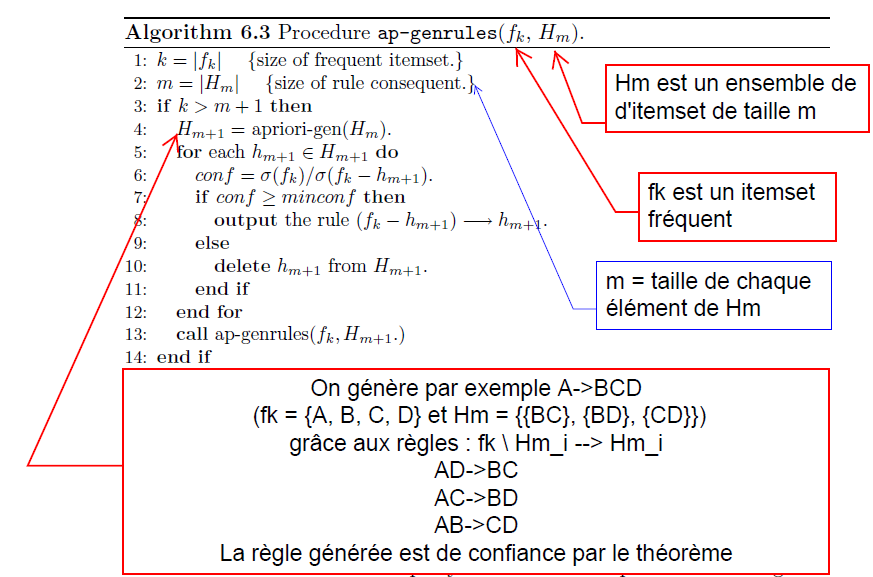
\includegraphics[scale=0.75]{Images/conf_algo2}
				\caption{Génération de règles de confiance à}
				partir de règles de confiance plus petites.
				\label{fig:conf:algo2}
			\end{figure}\noindent
			%
		%
	%
	\newpage
	%
	\section{Représentations compactes des itemsets fréquents}
		\alinea Le nombre de transaction en pratique peut être très élevé.
			C'est pourquoi il est utile de rendre compact l'ensemble
			des itemsets fréquents.
		%
		\subsection{Maximal Frequent Itemset}
			\begin{tabular}{lp{10cm}}
				\myul{\textbf{\hl{Maximal Frequent Itemset}}} & 
					\red{Itemset fréquent pour lequel aucun de ses 
					super-ensembles immédiat ne sont fréquents.}
			\end{tabular}~\\
			%
			\begin{figure}[H]
				\centering
				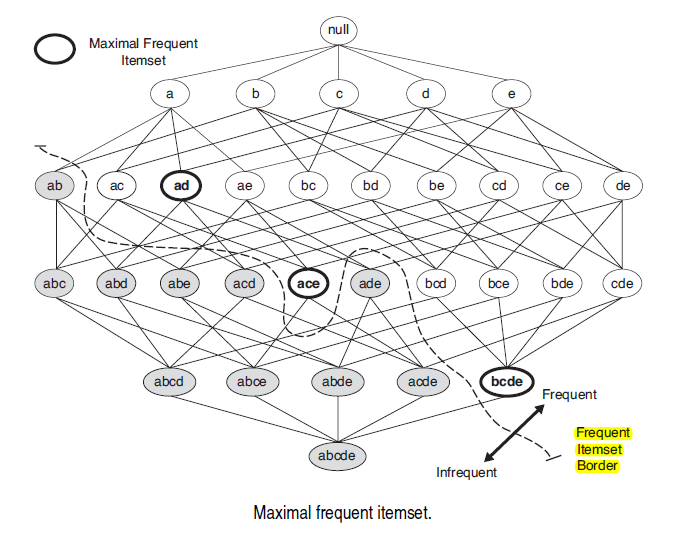
\includegraphics[scale=0.90]{Images/max_item_set.png}
				\caption{}
				\label{fig:max_it_set}
			\end{figure}\noindent
			%
			\alinea On voit ici qu'on peut se limiter à donner les itemset
				en gras sur la figure \ref{fig:max_it_set}, car en prenant
				tous leurs sous-ensemble, on obtient tous les itemsets 
				fréquents. La \myul{\textbf{\hl{limitation}}} de cette
				représentation est qu'on
				abandonne le support count des sous-ensembles, ce qui
				est embêtant pour calculer la \textit{confidence} des
				règles générées par ces premiers.
			%
		%
		\subsection{Closed Frequent Itemsets}
			\alinea Cette représentation propose un \hl{ensemble compact
				sans abandonner le support count des itemset.}\\
			%
			\begin{tabular}{lp{14cm}}
				\myul{\textbf{\hl{Closed Itemset}}} &
					\red{Un itemset $X$ est fermé si aucun des super-ensembles
						 immédiats de $X$ n'a exactement le même support 
						 count que $X$.}
			\end{tabular}~\\~\\
			%
			\alinea On peut donc noter que si $\{A\}$ est non-fermé,
				alors, il existe un objet $C$ t.q. la règle 
				$A \longrightarrow C$ a 
				une confiance de 100\%. En effet, si $\{A\}$ n'est pas fermé, 
				ça veut dire qu'il y a un autre objet ($C$) t.q. 
				$A$ n'apparaît jamais sans $C$.\\
			%
			\alinea En effet, le fait d'avoir le
				même support count pour un super-ensemble veut dire que
				ce super-ensemble revient autant de fois dans les transactions
				que l'ensemble. \\
			%
			\textbf{Exemple} : Si on a $\sigma(\{X, Y\}) = 9$ et qu'on
				a $\sigma(\{X, Y, Z\}) = 9$, ça veut dire qu'à chaque
				fois qu'on a $\{X, Y\}$ dans une transaction, $Z$ est
				également présent. On peut donc déduire que la confiance
				(\textit{confidence}) de la règle $\{X, Y\} \longrightarrow Z$
				est de 100\%.\\~\\
			%
			\begin{tabular}{lp{12.15cm}}
				\myul{\textbf{\hl{Closed Frequent Itemset}}} & 
					\red{Un itemset est fermé et fréquent s'il est fermé
					et que son support dépasse $minsup$.}
			\end{tabular}~\\
			%
			\begin{figure}[H]
				\centering
				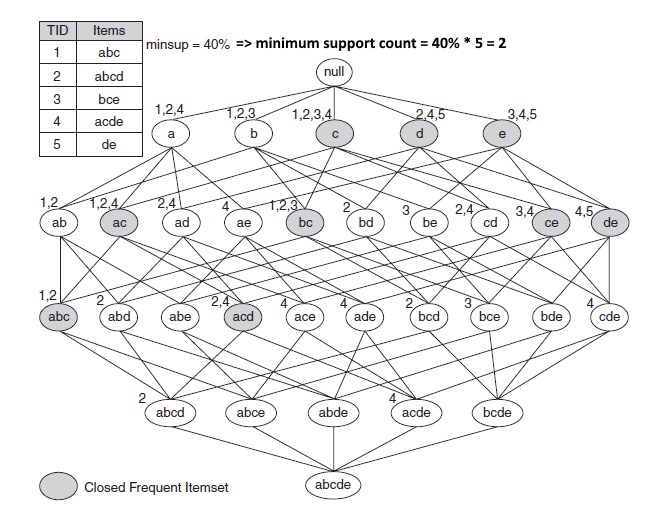
\includegraphics[scale=0.85]{Images/closed_itemset.png}
				\caption{}.
				\label{fig:closed_itemset}
			\end{figure}\noindent
			%
			\alinea Le support count des itemsets fréquents fermés 
				est sauvegardé dans la représentation.\\
			%
			\alinea L\hl{e support count de n'importe quel itemset fréquent
				non-fermé peut être obtenu en prenant le \textbf{max} 
				des support count de ses super-sensembles direct}. 
				L'\hl{algorithme} retrouvant le support count de tous les
				itemsets fréquents \hl{démarre donc de la plus grande taille 
				de d'itemsets fréquents}. En effet, l'algorithme a besoin
				de connaitre le support count des super-ensembles avant
				de passer aux sous-ensembles.\\
			%
			\textbf{Preuve} : si $\{a, b\}$ est ouvert, on sait qu'il y
				a un de ces super-ensembles immédiats qui a exactement
				le même support count que lui (par la définition de non-fermé). 
				La question serait alors de savoir duquel il s'agit. Mais
				on sait que le support count d'un super ensemble ne peut 
				pas être plus grand que le support count de l'ensemble 
				lui-même (anti-monotonicité). Donc, le max des support count
				de ses super-ensembles immédiats sera son propre support count.
				\\			
			%
			~\\
			%
			\alinea On peut noter que \hl{des règles peuvent être 
				détectées comme
				redondantes} grâce à cette notions d'itemsets fréquents fermés.
				En effet, si $\{b\}$ n'est pas fermé, mais que $\{b, c\}$
				l'est, la règle $\{b\} \longrightarrow X$ est redondante
				car elle a le même \textit{support} et la même
				\textit{confidence} que la règle $\{b, c\} \longrightarrow X$.
				Ces règles redondantes ne sont donc pas générées.
			%
			\begin{figure}[H]
				\centering
				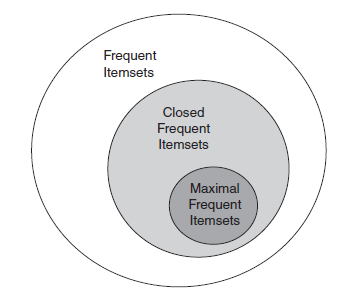
\includegraphics[scale=1.0]{Images/sets}
				\caption{Si un ensemble est maximal, il est forcément fermé}
				car sinon, il aurait un ensemble maximal comme super-ensemble
				(contradiciton).
				\label{fig:sets}
			\end{figure}\noindent
			%
		%
	%
	\newpage
	%
	\section{Optimiser Apriori}
		\alinea \hl{Bien que déjà pas mal, l'algorithme Apriori fait beaucoup
			d'accès à la base de données quand il compte les support count.}
			De plus, lorsque les largeurs de transaction augmentent, le
			temps de calcul augmente aussi de manière significative.
			Nous allons donc voir quelles sont les \hl{améliorations} 
			que nous pouvons apporté à l'ordre dans lequel les itemsets
			sont parcourus \hl{lors de la sélection des itemsets fréquents}..
		%
		\subsection{Traverser un treillis}
			\alinea Le treillis formé par les itemsets de l'ensemble des 
				transactions peut être traversé afin d'y trouver les 
				itemsets fréquents. Tout repose alors sur la technique
				de recherche utilisée. Quelques unes de ces stratégies 
				sont expliquées ci-dessous.
			%
			\begin{figure}[H]
				\centering
				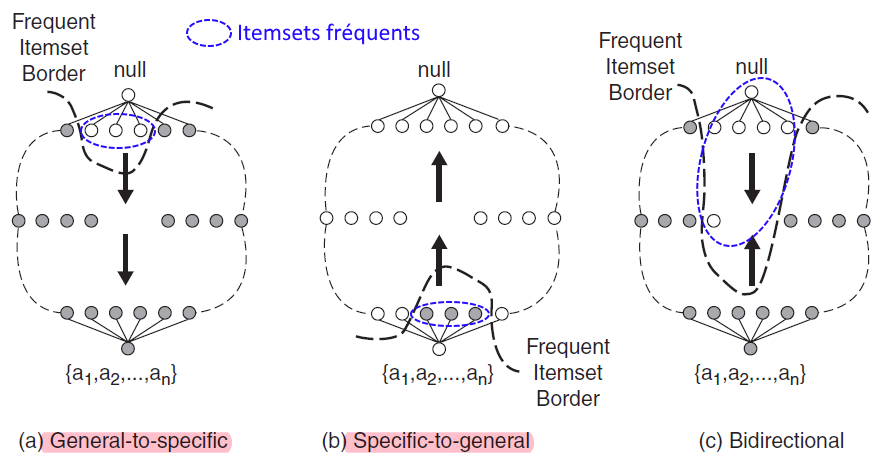
\includegraphics[scale=0.65]{Images/lattice_1.PNG}
				\caption{}
				\label{fig:lattice:1}
			\end{figure}\noindent
			%
			\subsubsection{\hl{General-To-Specific}}
				\alinea On démarre de petits itemsets 
					(1 éléments, puis 2, ...) pour terminer dans les
					grands itemsets.
					Cette méthode est efficace lorsque les itemsets 
					fréquents sont petits. Dés lors, la frontière
					fréquents/non-fréquents se trouve en haut du treillis
					(cf. figure \ref{fig:lattice:1}).
				%
			%
			\subsubsection{\hl{Specific-To-General}}
				\alinea \`A l'inverse de la recherche précédente, on 
					démarre cette fois des grand itemsets pour terminer
					dans les plus petits. Cette méthode est efficace 
					lorsque les itemsets fréquents sont grands, et donc
					généralement \hl{quand on a de grandes transactions.} 
					Dés lors, la frontière
					fréquents/non-fréquents se trouve en bas du treillis
					(cf. figure \ref{fig:lattice:1}).
				%
			%
			\subsubsection{Bidirectionnel}
				\alinea On peut combiner les deux techniques précédentes,
					mais ça demande plus d'espace mémoire pour l'exécuter.
					Utile pour les transactions de tailles très variantes
					(beaucoup de grandes transaction et beaucoup de petites).
				%
			%
			\subsubsection{Classes d'équivalence}
				\alinea Pour parcourir le treillis plus efficacement,
					les objets peuvent y être regroupé par classes
					d'équivalence, c'est-à-dire par une propriété que
					tout le groupe a en commun, comme un \hl{préfixe} ou 
					un \hl{suffixe}. \hl{On peut noter que l'algorithme 
					\textit{Apriori} considérait les classes d'équivalence
					de taille}. On y prenait donc d'abord tous les itemsets
					de taille 1, puis on passait à ceux de taille 2, ...
				%
				\begin{figure}[H]
					\centering
					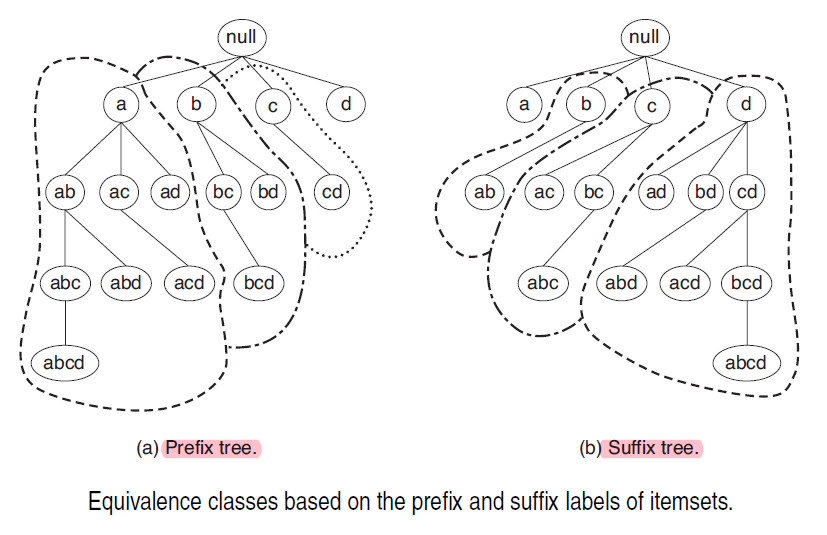
\includegraphics[scale=0.65]{Images/lattice_2.png}
					\caption{}
					\label{fig:lattice:2}
				\end{figure}\noindent
				%
			%
			\subsubsection{Profondeur / Largeur}
				%
				\begin{figure}[H]
					\centering
					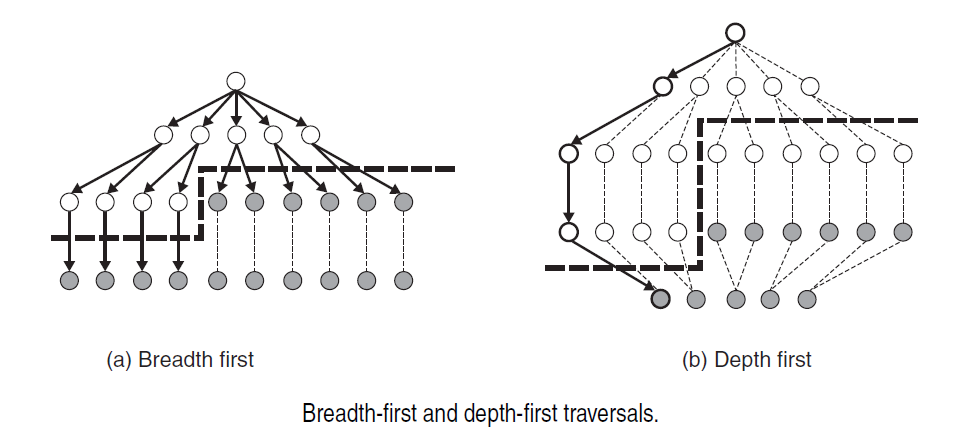
\includegraphics[scale=0.65]{Images/lattice_3}
					\caption{}
					\label{fig:lattice:3}
				\end{figure}\noindent
				%
				\alinea L'algorithme \textit{Apriori} traverse les 
					itemsets en largeur, considérant les tailles
					inférieurs et finissant dans les grandes tailles.\\
				%
				\alinea L'exploration en profondeur quand à elle est souvent
					utilisée en pratique car elle permet un grand élagage. 
					On peut élaguer de deux 
					manières, nous prendrons comme exemple la figure 
					\ref{fig:lattice:4}.
				%
				\begin{enumerate}
					\setlength{\itemsep}{0pt}
					\setlength{\parskip}{0pt}
					\setlength{\parsep}{0pt}
					\item \hl{Si un itemsets $X$ est trouvé fréquent, alors,
						tous les sous-arbres ne contenant que des 
						sous-ensembles de $X$ peuvent être ignorés pour 
						la suite de l'exploration}. Cet élagage utilise
						l'ordre lexicographique utilisé dans l'arbre.
						C'est l'exemple avec $\{b, c, d, e\}$. Par contre
						si $\{a, b, c\}$ est trouvé fréquent, on ne peut
						pas élaguer le sous-arbre $\{a, c\}$ car celui-ci
						contient des ensembles, comme $\{a, c, d, e\}$ 
						par exemple, qui ne sont pas des sous-ensembles de
						$\{a, b, c\}$.
					\item Si le support de $\{a, b, c\}$ est le même 
						que le support de $\{a, b\}$, on peut ignorer
						les sous-arbres qui ont $abd$ et $abe$ comme
						racine car \hl{on est certains qu'ils ne contiendront 
						pas d'itemsets fréquents maximaux}.\\
						\myul{\textbf{\hl{On peut le prouver}}}. En effet,
						si $\{a, b, c\}$ et $\{a, b\}$ ont le même support 
						count, ça veut dire que dans une transaction,
						$\{a, b\}$ n'apparaît jamais sans $c$. On a dés lors
						qu'$\{a, b, d\}$ a le même support que 
						$\{a, b, c, d\}$ qui aura été exploré dans le 
						sous-arbre de racine $\{a, b, c\}$ de par l'ordre 
						lexicographique respecté.
				\end{enumerate}
				%
				
				%
				\begin{figure}[H]
					\centering
					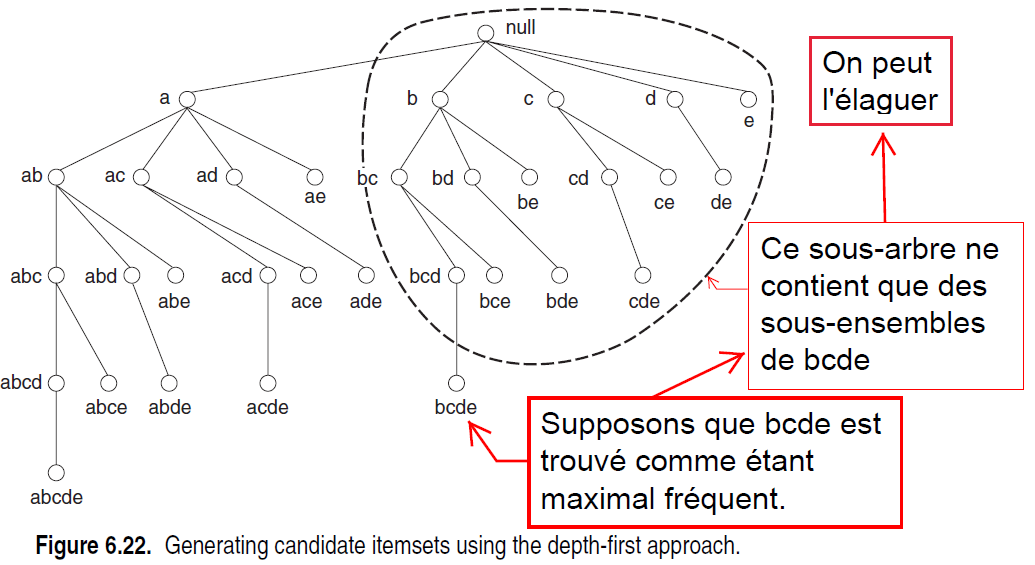
\includegraphics[scale=0.6]{Images/lattice_4}
					\caption{}
					\label{fig:lattice:4}
				\end{figure}\noindent
				%
			%
		%
		\subsection{Représentation des transactions}
			\alinea On peut aussi chercher à optimiser la structure de 
				données contenant les transactions. On distingue deux
				types principaux. Ils sont représentés sur la figure 
				\ref{fig:transactions}. La structure de gauche est généralement
				utilisée mais celle de droite a quelques avantages. En effet,
				la \textbf{\hl{structure verticale}} stocke, pour chaque objet,
				la liste des transactions dans lesquels l'objet est présent.
				\hl{Cependant, la liste des ID de transactions est parfois
				trop grandes que pour être stockée de cette manière.}
			%
			\begin{figure}[H]
				\centering
				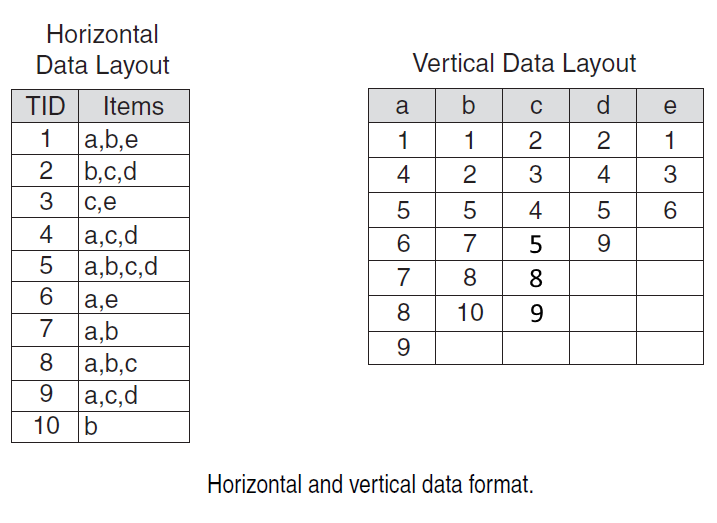
\includegraphics[scale=0.425]{Images/transactions}
				\caption{}
				\label{fig:transactions}
			\end{figure}\noindent
			%
			\alinea En partant d'une telle structure, il est aisé de définir
				des relations entre les objets et les itemsets dans lesquels
				ils sont contenus.	\\
			%
			~\\
			%
			\begin{tabular}{lp{12cm}}
				\textbf{\hl{cover($i$)}} &
					\red{Soit un item $i$, $cover(i)$ = l'ensemble des
						 transaction qui contiennent l'objet $i$.} Exemple,
						 dans la figure \ref{fig:transactions}, $cover(e)$
						 = $\{1, 3, 6\}$.\\
				\textbf{\hl{conditional cover, cocov($[s]$)}} & 
					\red{Soit un itemset $s$, et l'ensemble des objets $I$;
						\begin{align*}						
							cocov[s] = \{ (i, T) | 
								&i \in I, \textbf{et}\\							
								&i \text{ précède tous les él. de } s 
									\text{ dans l'ordre lex.}, \textbf{et}\\
								&T = cover(i \cup s) \}
						\end{align*}}
						Exemple, dans la figure \ref{fig:transactions}, \\
						  & $cocov[c] =  \{ (a, \{4, 5, 8, 9\}),
								(b,\ \{2, 5, 8\})\}$\\
						  & $cocov[be] = \{ (a,\ \{1\})\}$
			\end{tabular}~\\~\\~\\
			%
			On peut noter que pour $j \cup s$ un itemset, $j \in I$, alors
			$\forall i \in I,\ i\prec j$, on a
			$$ cocov[j \cup s](i) = cocov[s](j) \cap cocov[s](i) $$
		%
	%
	\newpage
	%
	\section{Algorithme FP-Growth}
		\alinea Cet algorithme utilise une structure de donnée un peu 
			qui s'appelle le FP-Tree.
		%
		\subsection{FP-Tree}
			\alinea Construire un FP-Tree comporte plusieurs étapes
			\begin{enumerate}
				\setlength{\itemsep}{0pt}
				\setlength{\parskip}{0pt}
				\setlength{\parsep}{0pt}
				\item On compte tout d'abord les support count des itemsets
					de taille 1, afin de \hl{trier les objets par ordre 
					décroissant} de support et pour écarte les non-fréquents.
				\item On passe ensuite une deuxième fois sur les transactions
					pour construire les branches du FP-Tree, c'est ce qui est
					montré sur la figure \ref{fig:fptree:1}. Cette étape
					\hl{trie les transactions par préfixe commun, en
					coupant dans l'ordre des objets de l'étape 1.}.
			\end{enumerate}
			%
			\begin{figure}[H]
				\centering
				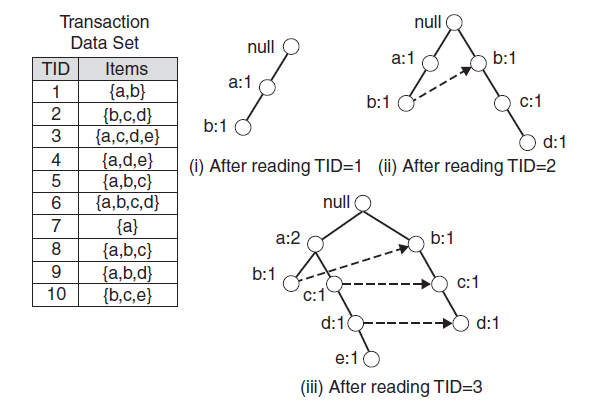
\includegraphics[scale=0.625]{Images/fptree_1a.png}
				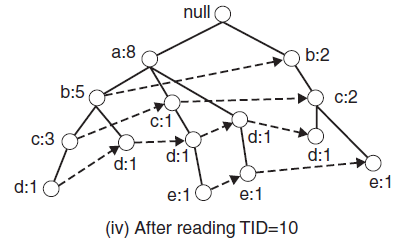
\includegraphics[scale=0.625]{Images/fptree_1b.png}
				\caption{}
				\label{fig:fptree:1}
			\end{figure}\noindent
			%
			On peut noter que l'ordre décroissant des objets de l'étape 1.
			ne garanti pas une taille minimum de l'arbre. De plus,
			dans le pire des cas, cette représentation prend plus de place
			que le dataset non compressé (pointeurs, compteurs, ...), mais
			en général, il le compresse tout de même.
			%
		%
		\subsection{Génération d'itemsets fréquents}
			\alinea\hl{ L'avantage de cette algorithme est de pouvoir déduire
				les itemsets fréquents directement depuis la structure
				de donnée.}
			%
			\subparagraph{Décomposition en sous-problème} On commence
				par explorer le FP-Tree de manière "bottom-up",
				donc, dans l'exemple, de $e$ à $a$, et on le divise 
				en sous-problème, comme l'illustre la figure 
				\ref{fig:fptree:2}. C'est ici que les pointeurs entre
				objets vont être utiles. En effet, dés qu'on tombe
				sur un $e$ dans l'arbre, on peut suivre les pointeurs
				pour trouver tous les autres $e$.
			%
			\begin{figure}[H]
				\centering
				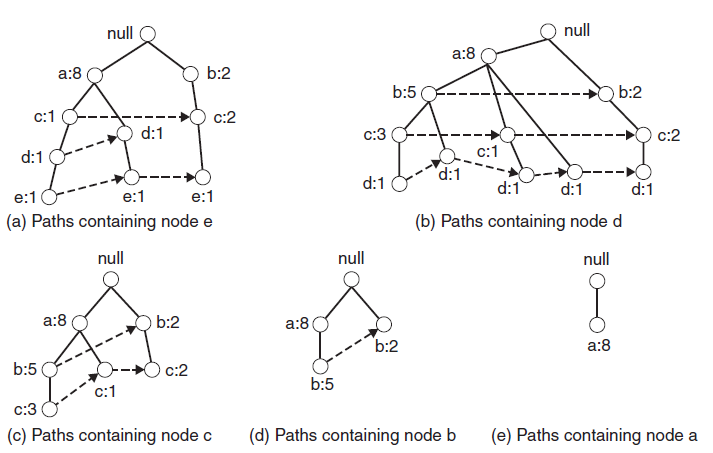
\includegraphics[scale=0.6]{Images/fptree_2.png}
				\caption{}
				\label{fig:fptree:2}
			\end{figure}\noindent
			%
			\vspace*{-1cm}
			%
			\subparagraph{Division en FP-Tree conditionnel} On va ensuite
				regarder, suffixe par suffixe, quel itemsets sont fréquents
				pour chaque sous-problème.\hl{ L'obtention d'un FP-Tree 
				conditionnel se fait par $cocov$}, défini précédemment, 
				les ID de transaction étant remplacés par des chemins 
				de l'arbre. Ceci est illustré à la figure 
				\ref{fig:fptree:3}. \hl{On peut y remarquer que $b$ est
				supprimé de l'arbre (b)}. Ceci s'explique par le fait
				que $b$ ne se retrouve qu'une seule fois dans l'arbre (a)
				et le seul chemin partant de lui arrivant en $e$ a un 
				support count de 1, on en conclut donc que tout chemin 
				partant de $b$ vers $e$ est non fréquent. Comme chaque 
				sous-problème est disjoint, on ne génère pas d'itemsets
				dupliqués.
			%
			\begin{figure}[H]
				\centering
				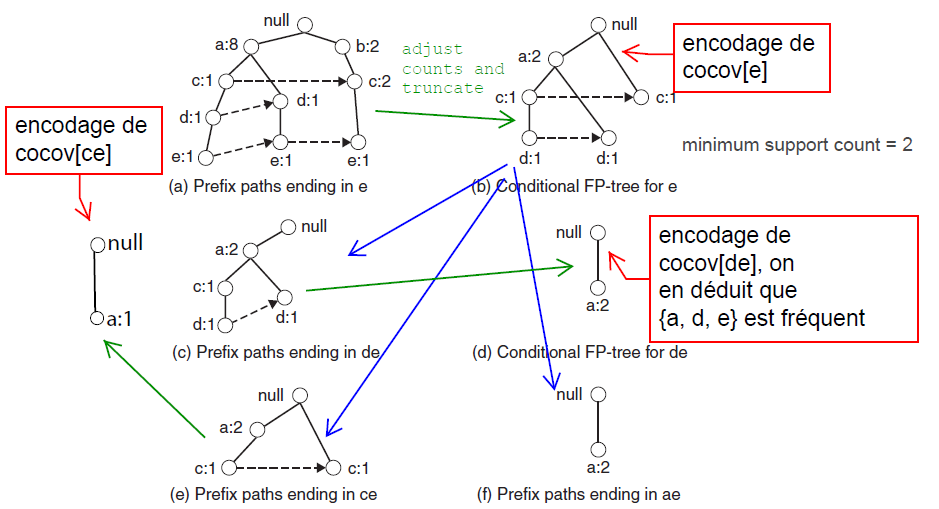
\includegraphics[scale=0.625]{Images/fptree_3}
				\caption{}
				\label{fig:fptree:3}
			\end{figure}\noindent
			%
		%
	%
%
\part{Analyse de clusters}
	\alinea \hl{Cette analyse divise les données en groupes (clusters), qui
		ont du sens, qui sont utiles, ou les deux.}
	%
	\paragraph{\point Buts du clustering}
		\subparagraph{\hl{Clustering pour la Compréhension}} Le clustering
			peut être utilisé pour classifier des objets, les clusters
			représentant les classes et le clustering étant la manière
			dont les objets sont classés. Ceci peut être utilisé en 
			biologie (hiérarchie, taxonomie, classer de l'ADN, ...), 
			en récupération d'information (recherche web, classement de
			données récupérées automatiquement, ...), dans la prévision
			climatique, en psychologie et en médecine (diagnostic, 
			analyse de la distribution de pathogènes, ...) ou enfin le 
			monde des affaires (informations sur les clients, comprendre
			les intérêts de groupes de personnes, ...).
		%
		\subparagraph{\hl{Clustering pour l'Utilité}} 
			\hl{Le clustering peut être
			utilisé pour trouver l'"individu type" (prototype) 
			d'un groupe de donnée.}
			En effet, on peut trouver, pour chaque cluster formé, l'individu
			qui représente le mieux le cluster. Cette approche est utilisée
			pour réduire un \hl{jeu de donnée (pour l'analyser, on se concentre
			sur l'individu le plus représentatif du jeu}), pour \hl{la 
			compression des données} (prendre l'image la plus représentative
			d'un ensemble d'image pour la compression vidéo, ...), ou encore
			pour trouver efficacement les plus proches voisins d'une
			donnée \hl{(si deux prototypes sont très éloignés, alors, les
			objets du premier cluster ne peuvent pas être plus proches
			voisins des objets du deuxième).}
		%
	%
	\section{Approche générale}
		\alinea Un clustering se base sur la notion de distances entre
			individus d'un jeu de données. Au plus des objets du sein
			d'un cluster sont proches, et au plus les clusters sont éloignés
			les uns des autres, au mieux on pourra distinguer les groupes
			de données.\\
		%
		~\\
		%
		\alinea De par la diversité des données que l'on peut traiter, 
			on ne peut donner une\hl{ définition claire d'un cluster qu'au
			cas par cas}. On peut néanmoins différencier une analyse
			de clusters d'une classification par le fait qu'une classification
			se base sur des labels connus à l'avance, tandis que l'analyse
			par cluster tire des groupes à partir des données uniquement, 
			c'est donc de la \hl{classification non-supervisée} (Ch. 4 = 
			classification supervisée car on donne des labels connus à 
			l'avance).
		%
		\subsection{Types de clustering}
			\alinea \hl{Un clustering est un groupe de clusters.} Il y a 
				plusieurs types de clustering.
			%
			\subsubsection{Clustering à partitions}
				\alinea Les clusters sont simplement des p\hl{artitions 
					disjointes} du jeu de données, où chaque objet
					peut être rangé dans un et un seul cluster (partition).
					\hl{On parle alors de clustering exclusif}, car
					on n'a jamais qu'un objets appartient à deux clusters
					différents.
				%
			%
			\subsubsection{Clustering hiérarchique}
				\alinea Si on permet à un cluster d'avoir des 
					\hl{sous-clusters},
					on peut les organiser en \hl{arbre} et avoir un clustering
					dit "hiérarchique". On peut voir ce type comme
					séquence de clustering à partitions.
				%
			%
			\subsubsection{Clustering imbriqués (overlapping)}
				\alinea Si on permet à un objet d'appartenir à \hl{plusieurs
					clusters en même temps}, on parle de clustering
					"overlapping".
					On place alors les objets dans des clusters de "qualité
					égale" pour chaque objet.			
				%
			%
			\subsubsection{Clustering flou (fuzzy, probabilistic)}
				\alinea Ce type de clustering donne une probabilité par cluster
					pour un objet d'appartenir à chacun des cluster.
					On a donc un \hl{poids entre 0 et 1} pour chaque cluster
					pour chaque objet, mais \hl{la somme des poids d'un objet
					fait toujours 1}.\hl{ On peut noter qu'on n'autorise pas un 
					objet à appartenir à plusieurs classes en même temps}.
					En effet, on va généralement réduire un tel clustering à un
					clustering à partitions, où on place chaque objet dans le
					cluster pour lequel il a le poids le plus élevé.
				%
			%
			\subsubsection{Clustering complet}
				\alinea \hl{Chaque objet est répertorié dans un cluster}, même
					si ce premier est assez éloigné du centre du cluster.
				%
			%
			\subsubsection{Clustering partiel}
				\alinea Un objet n'est \hl{pas obligé d'être répertorié} 
					dans un
					cluster. En effet, \hl{un objet pourrait être du bruit
					et n'appartenir en fait à aucune des classes} formées
					par les clusters.
				%
			%
		%
		\newpage
		%
		\subsection{Types de clusters}
			\alinea Il existe plusieurs types de clusters, illustrés
				sur la figure \ref{fig:clusters}.
			%
			\begin{figure}[H]
				\centering
				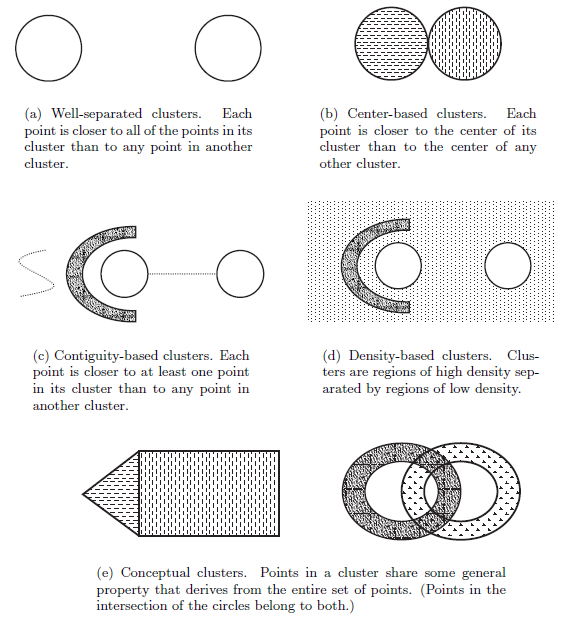
\includegraphics[scale=1.1]{Images/clusters.png}
				\caption{}
				\label{fig:clusters}
			\end{figure}\noindent
			%
			\subsubsection{Bien séparés}
				\alinea \hl{Cluster dans lequel chaque objet est plus proches
					de chacun des autres objets du cluster que de n'importe
					quel autre objet d'un autre cluster}. Définition
					satisfaite uniquement si le jeu de données contient des
					classes naturelles qui seront révélées par le clustering.
				%
			%
			\subsubsection{Basés sur un protoype (centre)}
				\alinea \hl{Cluster dans lequel chaque objet est plus proches
					du protoype qui défini le cluster cluster que de n'importe
					quel autre protoype}. Un prototype peut être défini
					comme :\\~\\
				%
				\begin{tabular}{lp{12cm}}
					\myul{\textbf{\hl{centroid}}} & 
						\red{Centre calculé sur la moyenne de tous les
							 membres du cluster}\\
					\myul{\textbf{\hl{medoid}}} &
						\red{Membre du cluster (\hl{donnée réelle}), le plus 
							 proche du centre, de la moyenne.} C'est donc le 
							 \hl{point le plus représentatif} du cluster.					
				\end{tabular}
				%
			%
			\subsubsection{Basés sur un graphe}
				\alinea Chaque objet est un noeud, et \hl{les clusters sont
					des composantes connexes}, il n'y a pas de lien
					entre deux clusters, mais tous les objets d'un
					même cluster sont connectés entre-eux. On parle 
					de \hl{"contiguity-based"} cluster quand il n'y a un lien
					que si les deux objets connectés sont situés dans une
					intervalle de distance défini.
				%
			%
			\subsubsection{Basés sur la densité}
				\alinea Chaque cluster est une région dense d'objet, 
					qui est entourée de régions moins denses.
				%
			%
			\subsubsection{Partageant une propriété (clusters conceptuels)}
				\alinea Cette définition englobe toute les autres, étant
					donné que deux objets appartiennent au même cluster
					s'ils partagent une propriété. Il reste à définir
					cette propriété (distance d'un centre, distance
					entre eux, stackés, ...). Une définition \hl{trop complexe}
					de cette propriété nous emmènerait dans le domaine
					du \textit{\hl{pattern recognition}}.
				%
			%
		%
	%
	\newpage
	%
	\section{K-Means}
		\alinea Il s'agit d'un algorithme donnant des \hl{clusters basés
			sur des prototypes}, formant un \hl{clustering à partitions},
			et utilisant des \hl{centroids} comme prototype de cluster. 
			L'algorithme peut être utilisé sur n'importe quel type de données
			permettant la définition d'une mesure de distance. 
			\hl{$K$ est le nombre de cluster voulu}. K-medoids correspond
			à K-means dans lequel on a remplacé les centroids par des
			medoids.\\
		%
		\alinea Les notations utilisées sont les suivantes :\\
		\begin{center}
			\begin{tabular}{|c|l|}
				\hline
				Symbole & Description\\
				\hline
				$x$ & Un objet.\\
				$C_i$ & Le $i^{\text{ème}}$ cluster.\\
				$c_i$ & Le centroid du cluster $C_i$.\\
				$c$ & Le centroid de tous les points.\\
				$m_i$ & Le nombre d'objets dans le $i^{\text{ème}}$ cluster.\\
				$m$ & Le nombre d'objets dans le jeu de données.\\
				$K$ & Le nombre de cluster.\\
				\hline			
			\end{tabular}
		\end{center}
		%
		\subsection{K-Means basique}
			\begin{figure}[H]
				\centering
				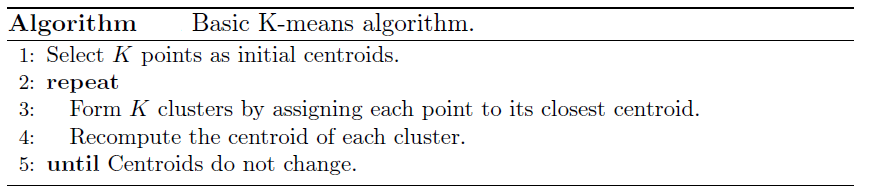
\includegraphics[scale=0.7]{Images/k-means_algo.png}
				\caption{L'algorithme basique pour K-Means}
				\label{fig:kmeans:algo:basic}
			\end{figure}\noindent
			%
			\alinea En choisissant les bonnes combinaisons de mesures 
				de proximités et les types de centroids, K-Means 
				converge toujours à une solution.
				\hl{L'étape 5 est souvent remplacée par une condition
				plus souple} (e.g. ne change plus à 1\% près).
				\hl{L'algorithme est linéaire en $m$, et est efficace si 
				$K$ est significativement plus petit que $m$.}
			%
			\subsubsection{Assigner des points à un cluster}
				\alinea On a besoin d'une notion de distance
					pour trouver le centroid le plus "proche".
					\hl{Cette notion doit être la plus simple possible} 
					car on va faire beaucoup de comparaisons.
				%
			%
			\subsubsection{Choisir le nouveau centroid}
				\alinea Chaque notion de distance vient avec sa fonction
					objectif. \hl{Le centroid choisi sera le résultat de la
					fonction objectif de la distance sélectionnée.}
				%
				\subparagraph{Données Euclidiennes} La fonction objectif
					de la \textbf{distance Euclidienne} est la minimisation
					de la somme des erreurs carrées (\hl{SSE}).
					$$ \text{SSE} = 
						\sum_{i=1}^{K}\sum_{x\in C_i} dist(c_i, x)^2 $$
					On peut alors montrer que le \hl{centroid qui minimise 
					cette erreur} est la moyenne (\hl{mean}).
					$$ \text{mean} = c_i = \frac{1}{m_i}\sum_{x\in C_i} x $$
					On peut noter que cette minimisation n'est pas optimale
					pour tout le jeu de données. C'est un optimal local
					pour les clusters et centroids choisi jusqu'à présent.\\
					La distance de \hl{Manhattan}\footnote{Distance en
					escalier, somme de la longueur de chaque marche} 
					\hl{quand à elle va minimiser le médian des points du
					cluster.}
				%
				\subparagraph{Documents écrits} On suppose que les données
					sont placées dans des "document-term matrix". 
					On cherchera ici a maximiser la cohésion des
					documents
					$$ \text{Total Cohesion} = 
						\sum_{i=1}^{K}\sum_{x\in C_i} cosine(c_i, x) $$
					\begin{figure}[H]
						\centering
						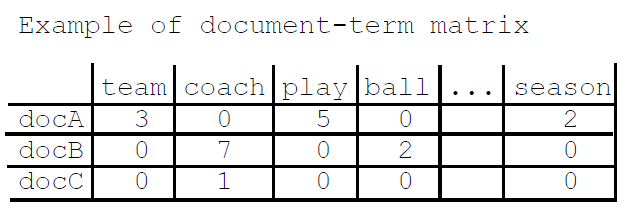
\includegraphics[scale=0.5]{Images/document.png}
						\caption{}
						\label{fig:document-term}
					\end{figure}\noindent
				%
			%
			\newpage
			%
			\subsubsection{Choisir les centroids initiaux}
				\subparagraph{Centroids aléatoires}	
					Une \textbf{première technique} est de
					faire plusieurs itérations en choisissant
					les centroids au hasard, et on garde l'itération
					qui minimise la SSE. \hl{Si on commence avec deux
					centroids initiaux par pair de cluster, alors
					ces centroids convergeront vers les vrais clusters}.
					En pratique, la probabilité que ca arrive avec des grands
					jeux de données est faible.
				%	
				\subparagraph{Clustering hiérarchique} Une autre technique
					est de commencer avec un clustering hiérarchique,
					et, prendre le clustering à k centres, et commencer avec
					ces k centres. En pratique, c'est couteux en calcul,
					et il faut que K soit petit par rapport à la taille
					du jeu de données.
				%		
				\subparagraph{Farthest-first-traversal} Sélectioner
					le premier point au hasard (ou prendre la moyenne 
					générale) et \hl{pour chaque centroid initial suivant,
					prendre le point le plus éloignés\footnote{%
					La distance est ici définie comme la distance minimale
					entre un point et les centroid déja choisi. On 
					maximise donc cette distance minimale} 
					des centroids déja
					choisis}. Le problème est que l'on pourrait sélectionner
					du bruit comme centroid, et s'éloigner des vrais clusters.
					On préfèrera donc prendre des groupes de points plutôt
					que des points, un groupe aura moins de chance d'être du
					bruit. Une fois que l'on a obtenu $k$ clusters, si on 
					prend le point le plus éloigné de tous les prototypes,
					on obtient un point d'un cluster existant 
					(\hl{\textbf{pigeon hole principle}}) et \hl{le rayon
					maximal de tous les cluster est défini par la distance
					entre ce point et son prototype de cluster.}
				%
			%
		%
		\subsection{Autres problèmes}
			\alinea Ci-dessous seront listés quelques problèmes qu'il reste
				à résoudre pour rendre l'algorithme robuste.
			%
			\subsubsection{Bruit}
				\alinea Pour éviter que le clustering soit influencé
					par le \hl{bruit, il peut être utile de le détecter et
					de le supprimer}. \hl{Il est à noter que pour certaines
					techniques de clustering, le bruit \textbf{n'est pas} à 
					supprimer.} Une technique serait de faire une première
					passe sur les données et de noter la contribution
					de chaque point à la SSE, et de supprimer les points
					induisant la plus grande erreur.
				%
			%
			\subsubsection{Réduire la SSE en postprocessing}
				\alinea Une manière simple de réduire la SSE est d'augmenter
					$K$ afin de réduire la distance entre les points et leur
					centroid, mais en pratique on ne veut pas augmenter le
					nombre de clusters.\\
				%
				\alinea On peut noter que la SSE total est la somme de
					la SSE apportée par chaque cluster.\\
				%
				~\\
				%
				\point On a donc \hl{deux
					techniques permettant de réduire la SSE en augmentant
					le nombre de clusters}.
				%
				\subparagraph{Diviser un cluster} Le cluster amenant la
					plus grande erreur.
				%
				\newpage
				%
				\subparagraph{Placer un nouveau centroid} On ajoute
					un nouveau cluster, dont le centroid sera le point le 
					plus éloigné de tout les autres.\\
				~\\~\\
				%
				\point \hl{Deux techniques réduisant la SSE en réduisant le
					nombre de cluster sont les suivantes.}
				%
				\subparagraph{Disperser un cluster} On dissout le cluster
					amenant le plus d'erreur et on réparti ses éléments dans
					les autres clusters.
				%
				\subparagraph{Fusionner deux clusters} Les clusters
					dont les centroids sont les plus proches l'un de l'autre
					sont fusionnés.
				%
			%
			\subsubsection{Mettre à jour les centroids}
				\alinea Mettre à jour les centroids après chaque ajout
					d'un élément à un cluster implique de vérifier
					aussi si ses éléments proches ne doivent pas changer 
					de cluster (est-ce que le centroid mis à jour
					est plus proche que le centroid actuel de l'objet ? Si
					oui, il faut le changer de cluster).\hl{ Une mise à jour 
					incrémentale évite d'avoir des clusters vides.}\\
				%
				\alinea Le point négatif est que cela induit \hl{une dépendance
					sur l'ordre} dans lequel les objets sont placés dans
					les clusters. Pour y remédier, on va rendre cet ordre 
					aléatoire.
				%
			%
		%
		\subsection{Bisecting K-Means}
			\begin{figure}[H]
				\centering
				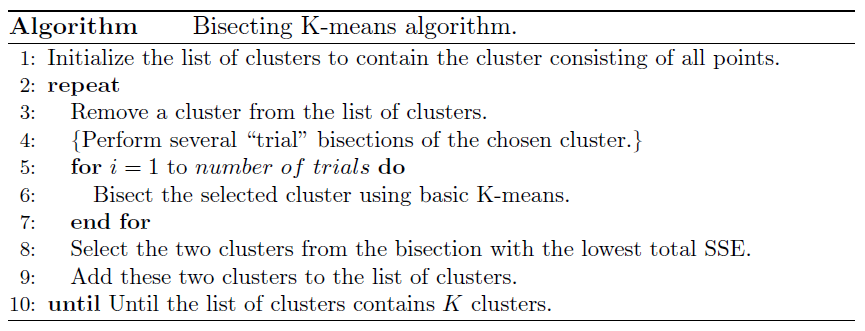
\includegraphics[scale=0.7]{Images/bisecting_k-means_algo.png}
				\caption{}
				\label{fig:k-means:bissecting:algo}
			\end{figure}\noindent
			Entre l'étape 8 et 9, on va raffiner le clustering choisi, en 
				réappliquant le K-Means basique avec les centroids
				du clustering
				choisi à l'étape 8.\hl{ Ceci permettra d'avoir un optimum
				local.}
				\hl{On peut utiliser cet algorithme pour faire un clustering 
				hiérarchique, en sauvegardant chaque étape.}
			%
		%
		\subsection{Types de cluster problématiques}
			\begin{figure}[H]
				\centering
				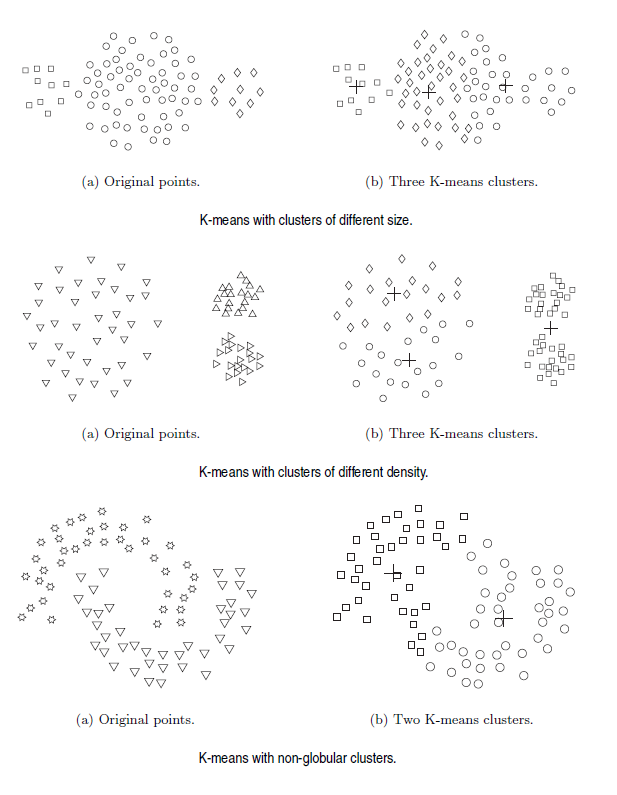
\includegraphics[scale=0.85]{Images/k-means_difficulties.png}
				\caption{}
				\label{fig:k-means:difficulties}
			\end{figure}\noindent
			%
			Le problème avec les types de clusters ci-dessus est que 
				\hl{la fonction
				objectif ne colle pas avec la définition des clusters} 
				qui ne sont
				pas bien séparés. De plus, pour les données ne permettant pas
				vraiment de définir un centroid, il faut préférer le 
				\hl{K-Medoid}.
			%
		%
		\subsection{K-Means comme problème d'optimisation}
			\alinea \hl{On pourrait chercher, parmi toutes les possibilités de 
				clustering, celle qui satisfait le mieux la fonction objectif.}
				Le problème étant que c'est infaisable à cause du nombre 
				de calcul 
				à faire. Une méthode d'approximation est la méthode gloutonne,
				qui choisit à chaque étape le choix qui a le meilleur score.\\
			%
			\alinea On peut de cette manière vérifier que c'est bien 
				le centroid	à la moyenne qui permet de minimiser la SSE.\\
			%
			~\\
			%
			\alinea On peut également changer de distance et de fonction 
				objectif. Si on prend la distance de Manhattan ($L_1$) 
				et la somme des erreurs absolues (SAE).
				$$ \text{SAE} = \sum^{K}_{i=1} \sum_{x\in C_i} dist_{L_1}
						(c_i, x) $$
				Et en résolvant l'équation de minimisation pour $c_i$, 
				on trouve
				bien que le centroid qui minimise la fonction est le médian
				des donnée du cluster.
			%
		%
	%
	\section{Clustering hiérarchique agglomératif}
		\alinea Il y a deux manière de considérer un clustering hiérarchique.
		\\~\\
		%
		\begin{tabular}{lp{12cm}}
			\myul{\textbf{\hl{Agglomératif}}} & 
				\red{Commence le clustering en considérant chaque point
					 comme un cluster. Il y a donc $m$ clusters au départ,
					 et à chaque étape, on fusionne les clusters les
					 plus proches. Nécessite la notion de proximité de
					 entre clusters.}\\
			\myul{\textbf{\hl{Divisif}}} & 
				\red{Commence avec un seul cluster comprenant tous
					 les points et divise un cluster à chaque étape.}
		\end{tabular}~\\~\\
		On va donc discuter ici de la méthode agglomérative. On
		peut représenter le résultat d'un clustering hiérarchique avec 
		un dendrogramme (cf. figure \ref{fig:dendrogram}). La complexité
		est de $O(m^2log m)$ en temps et $O(m^2)$ en espace, ce qui est
		très couteux pour $m$ grand.
		%
		\begin{figure}[H]
			\centering
			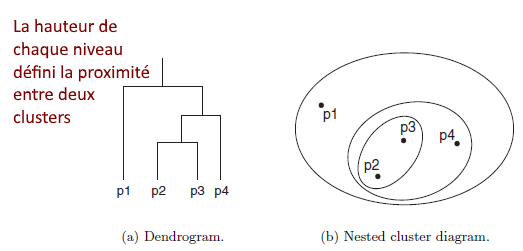
\includegraphics[scale=0.8]{Images/dendrogram.png}
			\caption{}
			\label{fig:dendrogram}
		\end{figure}\noindent
		%
		\subsection{Algorithme basique}
			\alinea En démarrant avec un cluster par objet, on a 
				l'algorithme suivant.
			\begin{figure}[H]
				\centering
				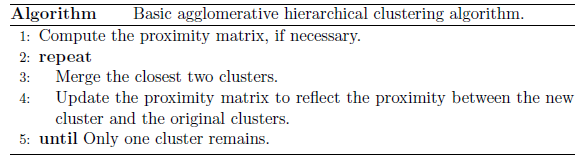
\includegraphics[scale=0.8]{Images/basic_hierarchical_algo.png}
				\caption{}
				\label{fig:hierarchical:basic_algo}
			\end{figure}\noindent
			%
			\alinea Il faut maintenant définir la notion de procimité entre
				clusters.
			%
			\subparagraph{Distances entre les objets} On peut définir la 
				proximité entre deux cluster, par la distance maximale (MAX),
				minimale (MIN) ou moyenne (group average = UPGMA)
				qui existe entre les différents
				points des deux clusters. Ceci est représenté sur la figure
				\ref{fig:hierarchical:distances}. On peut noter que
				MAX essaie de minimiser le diamètre des clusters, pour 
				qu'ils soient le plus groupés possible.
				\begin{figure}[H]
					\centering
					\includegraphics[scale=1.0]{Images/%
						hierarchical_distances.png}
					\caption{}
					\label{fig:hierarchical:distances}
				\end{figure}\noindent
			%
			\subparagraph{Distances entre prototypes} On peut aussi définir
				la proximité entre deux clusters comme la proximité entre 
				leur prototype respectif.
			%
			\subparagraph{Méthode de Ward} \hl{Un cluster est ici représenté
				par son centroid, elle mesure l'augmentation de SSE que
				résulte de la fusion de deux clusters.} Cette méthode
				est \hl{la seule} parmi celle présentées qui 
				\hl{peut réduire la	métrique de distance lorsqu'on 
				fusionne deux clusters}. C'est en réalité ce qui est
				utilisé en général dans le K-Means.
			%
		%
		\subsection{La formule de Lance-Williams}
			\alinea Cette formule permet de \hl{généraliser} toutes
				les définitions de proximité en une seule. Il suffit
				de modifier les paramètre de la formule pour passer
				d'une définition à l'autre. De plus, des \hl{algorithmes
				performants} utilisant cette formule existent.
			%
		%
		\subsection{Lacunes majeures}
			\alinea La principale lacune du clustering hiérarchique est
				qu'il est très gourmand en ressources, même si on utilise
				déjà des techniques d'approximation.
			%
			\subsubsection{Gérer les clusters de tailles différentes}
				\alinea Il peut être intéressant de considérer la taille
					des clusters que l'on souhaite fusionner. Les méthodes
					vues jusqu'à présent considèrent tous les clusters
					comme égaux, on a utilisé la méthode dite
					\textbf{unweighted}, on a pas mis de poids sur les 
					points. L'autre méthode, \textbf{weighted}, peut
					être utilisé dans le cas où les classes sont
					inégalement représentées. La distance "group average"
					a été adaptée aux deux méthodes. La unweighted
					est juste la moyenne des distances et est appelée
					UPGMA. La méthode weighted est quant à elle appelée
					WPGMA. Soit deux clusters $R$ et $Q$, où $R$ a été 
					formé en fusionnant $A$ et $B$.
					\begin{align*}
						\text{UPGMA}:&\ \ prox(R, Q) =&
							\frac{\sum_{{x \in R, 
							y \in Q}}dist(x, y)}%
								{m_R \cdot m_Q} \\
						\text{WPGMA}:&\ \ prox(R, Q) =&
							\frac{prox(A, Q) + prox(B, Q)}{2}
					\end{align*}
				%
			%
			\subsubsection{Les fusions sont finales}
				\alinea \hl{Une fois que deux clusters sont fusionnés, on ne
					peut plus en modifier les éléments. En effet, 
					Avec la méthode de Ward et en minimisant la SSE, 
					la fusion de deux clusters ne représente pas un
					minima local si l'on regarde à la SSE totale. }
					En effet, il se peut qu'un élément d'un cluster soit
					plus proche d'un centroid d'un autre cluster que le sien.
				%
			%
			\subsubsection{Forces et faiblesses}
				\alinea La raison principale de l'utilisation des
					algorithmes de clustering hiérarchiques est le
					besoin d'une hiérarchie, d'une taxonomie dans les
					donnée.
				%
			%
		%
	%
	\newpage
	%
	\section{DBSCAN}
		\alinea Cette technique \hl{produit un clustering basé sur la densité.} 
			Technique très efficace, sauf quand les clusters ont des densités
			très différentes entre eux, et quand les données ont 
			un grand nombre de dimensions (attributs).
		%
		\subsection{Densité}
			\alinea Pour définir la densité autour d'un point, on utilise 
				la méthode \hl{center-based}. Cette méthode consiste à compter
				le nombre de points contenu dans un rayon, \hl{$Eps$}, autour
				de ce point, le point se compte lui-même. Sa complexité 
				en temps est \\
				$O(m \times \text{temps pour trouver les
				voisins dans le rayon } Eps)$, ce qui veut dire qu'avec
				la bonne structure de donnée (KD-Tree, ...), on peut
				avoir une complexité en $O(m \log m)$.\\
			%
			~\\
			%
			\alinea En utilisant cette technique on peut alors classifier 
				un point comme étant un : 
				\begin{itemize}
					\setlength{\itemsep}{0pt}
					\setlength{\parskip}{0pt}
					\setlength{\parsep}{0pt}
					\item[(1)] \textbf{Core Point} : \red{à l'intérieur d'une
						région dense.} Un point est considéré comme tel
						si il y a au moins \hl{$MinPts$} dans un rayon 
						de $Eps$ autour de lui, lui y comprit.
					\item[(2)] \textbf{Border Point} : \red{sur le bord d'une
						région dense, il a un ou des Core Points dans un
						rayon de $Eps$ autour de lui.} 
						\hl{Un border point peut avoir jusqu'à $MinPts -1$
						Core Point dans son voisinage (rayon de $Eps$ autour de lui).}
					\item[(3)] \textbf{Noise/Background Point} : \red{dans une
						région peu occupée.} Il n'est ni un Core Point, ni
						un Border Point.
				\end{itemize}
			%
			\begin{figure}[H]
				\centering
				\includegraphics[scale=0.8]{Images/dbscan_eps.png}
				\caption{}
				\label{fig:dbscan:eps}
			\end{figure}\noindent
			%
		%
		\newpage
		%
		\subsection{Algorithme}
			\begin{figure}[H]
				\centering
				\includegraphics[scale=1]{Images/dbscan_algo.png}
				\caption{}
				\label{fig:dbscan:algo}
			\end{figure}\noindent
			%
			\subsubsection{Valeur des paramètres}
				\alinea Il faut maintenant fixer $MinPts$ et $Eps$.
					Supposons qu'un nombre $k$ soit fixé (\hl{en pratique, 
					DBSCAN prend k=4}), alors, on appelle $k-dist$ la 
					distance entre un point et son $k^{\text{ème}}$ voisin 
					le plus proche. Si on trie les points par ordre 
					croissant pour leur valeur de $k-dist$, on pourra
					normalement observer un changement brusque dans la 
					courbe, ce changement brusque représente 
					normalement la limite entre le non-bruit et le bruit.
					\hl{On prendra donc la valeur de $k-dist$ à ce changement
					brusque comme $Eps$ et $MinPts = k$.} Ceci est illustré
					à la figure \ref{fig:dbscan:k}.\\
					\begin{minipage}{0.475\textwidth}
						\begin{figure}[H]
							\centering
							\includegraphics[scale=0.8]{Images/dbscan_k.png}
							\caption{}
							\label{fig:dbscan:k}
						\end{figure}\noindent
					\end{minipage}\hfill
					\begin{minipage}{0.475\textwidth}
						\begin{figure}[H]
							\centering
							\includegraphics[scale=0.8]{Images/%
								dbscan_density.png}
							\caption{}
							\label{fig:dbscan:density}
						\end{figure}\noindent
					\end{minipage}\noindent~\\~\\
				%
			%
			\subsubsection{Problème de densités variables}
				\alinea \hl{Si des clusters ont des densités très différentes,
					on ne pourra pas les détecter tous en même temps.}
					En effet, comme on le voit sur la figure 
					\ref{fig:dbscan:density}, $A$ et $B$ sont beaucoup plus
					dense que $C$ et $D$. Si on arrive à distinguer $A$ et, 
					$B$, alors $C$ et $D$ sont considérés comme du bruit, 
					et si on arrive à discerner $C$ et $D$, $A$, $B$, et 
					le bruit dans leurs alentours risquent d'être confondu
					en un seul cluster.
				%
			%
		%	
	%
	\section{EM-clustering}
		\alinea Clustering basé sur les \hl{probabilités}. Il consiste 
			en l'algorithme suivant :
		%
		\begin{figure}[H]
			\centering
			\includegraphics[scale=0.65]{Images/EM_algo.png}
		\end{figure}\noindent
		%
		\begin{figure}[H]
			\centering
			\includegraphics[scale=0.65]{Images/EM_param.png}
		\end{figure}\noindent
		%
		\vspace*{-1.5cm}
		%
		\begin{figure}[H]
			\centering
			\includegraphics[scale=0.65]{Images/EM_a.png}
		\end{figure}\noindent
		%
		\vspace*{-1.5cm}
		%
		\begin{figure}[H]
			\centering
			\includegraphics[scale=0.65]{Images/EM_b.png}
		\end{figure}\noindent
		%
		\alinea Le principe est donc de créer \hl{deux distributions
			normales de 
			probabilités, $f(A)$ et $f(B)$, définies par leur
			$\mu$ et $\sigma$} respectifs (pour un exemple à 
			deux clusters, on en créerait plus pour plus de
			clusters), on veut ensuite maximiser la probabilité 
			qu'a un objet $x$ d'appartenir à un cluster. 
			L'étape 4 visant à 
			modifier le centre et le rayon de chaque cluster
			(et donc de chaque distributions) pour
			maximiser cette probabilité. On \hl{maximise donc
			le \textbf{log-likelihood}}, défini comme suit:
			\begin{figure}[H]
				\centering
				\includegraphics[scale=0.65]{Images/EM_log.png}
			\end{figure}\noindent
		%
		\alinea On peut noter que les \hl{dénominateurs de 
			$Pr(A | x)$ et de $Pr(B | x)$ sont les même}, 
			et on a donc pas besoin de les calculer.
		%
	%
	\newpage
	%
	\section{Clustering génétique}
		\alinea Comme tout algorithme génétique, ce
			clustering se base sur la définition de deux
			opérateurs : le \textbf{\hl{cross-over}} et 
			la \textbf{\hl{mutation}}.
		%
		\begin{figure}[H]
			\centering
			\includegraphics[scale=0.65]{Images/genetic_principle.png}
		\end{figure}\noindent
		%
		\begin{figure}[H]
			\centering
			\includegraphics[scale=0.65]{Images/genetic_operators.png}
		\end{figure}\noindent
		%
		\begin{figure}[H]
			\centering
			\includegraphics[scale=0.65]{Images/genetic_algo.png}
		\end{figure}\noindent
		%
	%
	\newpage
	%
	\section{\'Evaluation des clusters}
		\alinea Appelée aussi la \textbf{validation de cluster},
			l'\hl{évaluation}
			d'un cluster est \hl{importante car les algorithmes de clustering
			trouveront des clusters, même dans des données à priori non 
			classifiables.} On pourrait comparer le résultat des trois
			algorithmes vus et, si les clusters ne se ressemble pas 
			entre les trois, alors on en conclut que ce sont des données
			aléatoire, \hl{mais ça ne marche pas pour un grand nombre
			d'attributs}. \\
		%
		~\\
		%
		\alinea Voici les cinq problématiques de la validation de cluster.
		%
		\begin{enumerate}
			\setlength{\itemsep}{0pt}
			\setlength{\parskip}{0pt}
			\setlength{\parsep}{0pt}
			\item Déterminer si les données sont "clusterisables" ou si, 
				au contraire, elles ont un caractère aléatoire.
			\item Déterminer le nombre correct de clusters.
			\item \'Evaluer la qualité du clustering sans se baser
				sur des informations externes.
			\item \'Evaluer la qualité du clustering en se basant
				sur des informations externes, comme des labels connus
				pour chaque objet ou autre.
			\item Comparer deux clustering pour déterminer lequel 
				est le meilleur.
		\end{enumerate}
		On y distingue trois types de problèmes : \\~\\
		\begin{tabular}{lp{14cm}}
			\myul{\textbf{\hl{Non-supervisé}}}	& 
				\red{Mesure la qualité sans faire appel à des
					 ressources externes.} Ces mesures sont aussi 
					 appelées \textbf{internal indices}.
					 La SSE est une mesure non-%
					 supervisée. On distingue deux types principaux
					 de mesures non-supervisées : \textbf{cluster cohesion}
					 et \textbf{cluster separation}. Les problèmes 
					 1 à 3 sont non-supervisés.\\
			\myul{\textbf{\hl{Supervisé}}}	&
				\red{Mesure qui teste le clustering avec un ensemble 
					 d'informations externes (labels, ...).} 
					 Elles sont aussi appelées \textbf{external indices}.
					\hl{ L'\textit{entropy} est une mesure supervisée} car
					 elle compare la correspondance avec les labels
					 connus des objets. Le problème 4. est supervisé.\\
			\myul{\textbf{\hl{Relatif}}} & 
				\red{Mesure visant à comparer différents clustering 
					 ou clusters, \hl{elle peut être 
					 supervisée ou non-supervisée}.} Comparer deux 
					 cluster avec leur SSE respective est une mesure
					 relative. Le problème 5. est relatif.
		\end{tabular}
		%
		\subsection{Non-supervisée avec cohésion et séparation}
			\alinea De manière générale, on définit la validité d'un 
				clustering (totale) par rapport à une somme pondérée
				reprenant la validité de chaque cluster.
				$$ \text{validité totale} = \sum_{i=1}^{K} w_i\cdot
						 					   validity(C_i) $$
				où $validity$ peut être la cohésion, la séparation, 
				ou une combinaison des deux.\\ 
				Il reste donc à définir les mesures de cohésion et de
				séparation pour différents types de clustering.
				De manière générale, la \textbf{cohésion} est la
				mesure qui indique à quel point les éléments d'un
				cluster sont proches les uns des autres, tandis que
				la \textbf{séparation} indique à quel point
				les différents clusters sont isolés les uns des autres.\\
			%
			\alinea Ces mesures peuvent être utilisées pour évaluer
				un clustering entier ou un seul cluster. Un cluster
				avec une grande cohésion est à préférer, et une faible
				séparation indique le besoin de fusionner des clusters.
			%
			\subsubsection{Cluster basés sur des graphes}
				\alinea La cohésion est définie comme la somme des poids
					sur les liens entre les objets du cluster. La 
					séparation est définie comme la somme des proximités
					entre les objets des deux clusters. $proximity$ peut
					être une mesure de similitude ou de dissimilitude. 
					Cette mesure est reportée sur un \hl{graphe de proximité},
					dans lequel les noeud sont les objets et les liens
					ont comme poids la proximité entre les deux objets  
					qu'ils relient.
					\begin{align*}
						cohesion(C_i) &= \sum_{x\in C_i, y\in C_i}
								proximity(x, y)\\
						separation(C_i, C_j) &= \sum_{x\in C_i, y\in C_j}
								proximity(x, y)
					\end{align*}
				%
			%
			\subsubsection{Cluster basés sur les prototypes}
				\alinea Pour ce type, la cohésion est définie comme
					la somme des distances entre les objets du cluster 
					et le prototype du cluster. La séparation est la 
					proximités entre les prototypes des deux clusters.
					($c$ est le prototype global). \hl{Si on prend
					le carré de la distance Euclidienne comme mesure de 
					proximité, la cohésion devient alors la mesure de la
					SSE.}
					\begin{align*}
						cohesion(C_i) &= \sum_{x\in C_i}
								proximity(x, c_i)\\
						separation(C_i, C_j) &= proximity(c_i, c_j)\\
						separation(C_i) &= proximity(c_i, c)
					\end{align*}
					Lorsque la distance Euclidienne est choisie pour mesurer 
					la proximité, la mesure de séparation entre clusters
					se fait généralement par la SSB (somme des carrés
					entre les groupes).
					$$ \text{SSB Totale} = \sum_{i=1}^{K} m_i \cdot 
							dist(c_i, c)^2 $$
					On peut dériver cette formule pour l'exprimer en 
					fonction de $c_i$ et $c_j$, d'où les deux définitions
					de séparations données plus haut.
				%
			%
			\subsubsection{Mesures globales}
				\alinea \hl{On peut noter que n'importe quelle mesure 
					non-supervisée de validité de cluster peut être utilisée
					comme fonction objective d'un algorithme de clustering.}
				%
			%
			\subsubsection{Graphe vs prototypes}
				\alinea \hl{Les mesures de cohésions et de séparations des 
					cluster basés sur des graphes et des clusters 
					basées sur des prototypes paraissent fort différentes,
					mais pour certaines valeurs, elles sont équivalente.}
				%
			%
			\subsubsection{Lien entre Cohésion et Séparation}
				\alinea Il y a parfois un lien fort entre ces deux
					mesures. En plus, \hl{la somme entre la SSE et la SSB
					donne une constante appelée TSS} (somme totale des
					carrés), \hl{qui est la même pour tous les 
					clusterings possible au sein d'un jeu de données}.
					$$ \text{TSS} = \sum_{i=1}^{K} \sum_{x \in C_i} (x - c)^2
						   = \text{SSE} + \text{SSB} $$
					Pour rappel, \hl{\textbf{SSE}} est la 
					sommes des erreurs carrées et 
					mesure la séparation à l'intérieur 
					d'un cluster. \hl{\textbf{SSB}}
					est la somme des carrés entre cluster et mesure la
					séparation inter cluster. Enfin, 
					\hl{\textbf{TSS}} est la somme 
					totale des carrés et ne dépend pas de la manière
					dont les objets sont répartis dans les clusters.
				%
			%
			\subsubsection{Coefficient de silhouette}
				\alinea \hl{Le coefficient de silhouette combine la cohésion
					et la séparation.} $sil_i = \frac{b_i - a_i}%
					{\max(a_i, b_i)}$ .Le coefficient a donc deux composantes;
					$a_i$ et $b_i$, $a_i$ étant la distance 
					moyenne entre le point $i$ et les points de son cluster, 
					et $b_i$ étant la distance moyenne minimale 
					entre le point et les points d'un autre cluster.
					\hl{Minimiser $a_i$ c'est augmenter la cohésion,
					et maximiser $b_i$ c'est augmenter la séparation.}\\
				%
				\alinea	Ce coefficient varie entre -1 et 1.
					S'il est négatif, cela veut dire que $a_i$ est 
					plus grand que $b_i$.
					Ce la dénoterait donc que l'objet devrait se trouver
					dans l'autre cluster ayant servi au calcul de $b_i$.\\
				%
				\begin{figure}[H]
					\centering
					\includegraphics[scale=1.0]{Images/silhouette.png}
					\caption{}
					\label{fig:eval:silhouette}
				\end{figure}\noindent
				La silhouette d'un clustering peut être obtenu en faisant
				la moyenne de la silhouette de tous les points.
				%
			%
		%
		\subsection{Non-supervisée avec matrice de proximité}
			\alinea Le principe est de calculer la corrélation entre
				une matrice de proximité dite "idéale" et la vrai matrice.
				Pour chaque objet $i$, la case $i, j$ de la \hl{matrice
				\textbf{idéale} vaudra 1 si $i$ et $j$ sont dans le
				même cluster et 0 sinon.} Corrélation calculée au 
				dessous ou en dessous de la diagonale de la \hl{matrice},
				étant donné qu'elle est \hl{symétrique}. Au plus la
				corrélation est élevée, au mieux c'est. Pas très 
				bon en pratique pour des clusters basés sur la densité 
				ou "contiguity-based.\\
			%
			\alinea Il es généralement plus simple de travailler avec
				une mesure de similarité plutôt que de distance.
				On peut calculer la similarité $s$ entre deux 
				objets $i, j$ de la manière suivante :
				$$ s(i, j) = 1-\frac{dist(i, j) - dist_{min}}%
				{dist_{max} - dist_{min}} $$
			%
			\alinea On peut aussi visualiser la corrélation pour déterminer
				si il y bien des clusters clairs qui se dessine (cf. 
				figure \ref{fig:clustering:correl1}) qui indiquent
				que les données sont classifiables, ou qui sont
				plus \hl{diffus} (cf. figure \ref{fig:clustering:correl2})
				et donc qui reflètent un \hl{caractère aléatoire}.
			%
			\begin{figure}[H]
				\centering
				\includegraphics[scale=0.75]{Images/correl_1}
				\caption{Clusters clairs, facilement distinguable}
				\label{fig:clustering:correl1}
			\end{figure}\noindent
			\begin{figure}[H]
				\centering
				\includegraphics[scale=0.75]{Images/correl_2}
				\caption{Clusters diffus, données aléatoires}
				\label{fig:clustering:correl2}
			\end{figure}\noindent
		%
		\subsection{Non-supervisée sur les attributs}
			\begin{minipage}{0.4\textwidth}
				Le \hl{coefficient de Pearson} est une mesure
					linéaire des \hl{relations entre les attributs}.
				%
				$\overrightarrow{x}$ et $\overrightarrow{y}$ représentant
					les vecteurs de valeurs des attributs de deux 
					objets.\\
				%
				$\overrightarrow{x} = (x_1, x_2, \ldots, x_n)$, \\
				$\overrightarrow{y} = (y_1, y_2, \ldots, y_n)$
				%
			\end{minipage}\hfill
			\begin{minipage}{0.55\textwidth}
				\begin{figure}[H]
					\centering
					\includegraphics[scale=0.6]{Images/pearson.png}
				\end{figure}\noindent
			\end{minipage}
			%
		%
		\vspace*{-0.5cm}
		%
		\subsection{Non-supervisée pour clustering hiérarchique}
			\begin{tabular}{lp{13cm}}
				\myul{\textbf{\hl{Cophenetic distance}}} &
					\red{Distance entre deux objets défini par la 
						 \hl{proximité} à laquelle une technique de 
						 clustering hiérarchique agglomératif
						 \hl{met les deux objets dans le même cluster
						 pour la première fois.}} Autrement dit, 
						 si deux clusters éloignés d'une distance
						 $d$ l'un de l'autre sont choisis pour
						 être fusionnés, alors, la distance cohpenetic
						 entre les objets des deux cluster sera de $d$.\\
				\myul{\textbf{\hl{CPCC}}} &
					\red{\textbf{CoPhenetic Correlation Coefficient}, 
						corrélation entre les entrées de la matrice de
						 distance cophenetic et les entrées de la 
						 matrice de distances originale.} On l'utilise
						 pour comparer des techniques hiérarchiques
						 entre elles pour un même jeu de données. Le score
						 le plus haut est le mieux.
			\end{tabular}
			%
		%
		\vspace*{-0.5cm}
		%
		\subsection{Déterminer le nombre idéal de clusters}
			\alinea Observer la variation de la SSE ou du coefficient
				de silhouette en fonction du nombre de clusters permet
				d'avoir une idée sur le nombre idéal. En pratique,
				c'est parfois pas très clair...
			%	
			\vspace*{-0.5cm}
			\begin{figure}[H]
				\centering
				\includegraphics[scale=0.65]{Images/clusters_number.png}
				\caption{En reprenant l'exemple de la figure
				\ref{fig:eval:silhouette}} \hl{10 est le nombre idéal car
				il minimise SSE et maximise silhouette}.
				\label{fig:eval:clusters_number}
			\end{figure}\noindent
			%
		%
		\newpage
		%
		\subsection{Tendance au clustering}
			\alinea On peut évaluer la tendance qu'à un jeu de données à 
				avoir des clusters naturels \hl{sans y appliquer de 
				techniques de clustering}. On va pour cela appliquer
				des tests statistiques, comme la méthode de \textbf{Hopkins}.\\
			%
			~\\
			%
			\alinea Pour un nombre $p$ fixé, on va générer $p$ nombres
				aléatoire dans le jeu de données et sélectionner
				$p$ données du jeu de données initial. Si $u_i$ représente
				le distance entre le point $i$ du jeu aléatoire et son
				plus proche voisin \hl{dans le jeu donnée initial}, et $w_i$
				la distance entre le point $i$ du jeu de donnée initial
				et son plus proche voisin dans le jeu de donnée initial,
				$$ H = \frac{\sum_{i=1}^{p} w_i}{\sum_{i=1}^{p} u_i +
												 \sum_{i=1}^{p} w_i} $$
				Un jeu de donnée aura donc \hl{tendance au clustering pour
				un H proche de 0}. En effet, il faudrait que la plus proche
				distance à l'intérieur de jeu de données initial ($w_i$)
				soit plus petite (plus proche) que la plus proche distance
				entre les données aléatoire et le jeu de donnée initial
				($u_i$), qui est sensée être élevée (éloignée). Au contraire
				si $u_i$ tend vers 0 (distance proche avec les données 
				aléatoire), H tendra vers 1.
			%
		%
		\subsection{Mesures supervisées}
			\alinea On distingue deux types principaux de techniques :
				les \textbf{orientées classification} et les 
				\textbf{orientées similarités}.
			%
			\subsubsection{Mesures orientées classification}
				\alinea On y retrouve l'entropy, la pureté, la precision,
					le recall et la F-mesure. On vérifie donc que 
					les objets d'un même cluster ont le même label de
					classe.\\~\\
				%
				\begin{tabular}{lp{15.25cm}}
					\myul{\textbf{\hl{Entropy}}} & 
						\red{On commence par calculer la distribution
							 des classes, i.e. $p_{ij}$ la probabilité
							 que l'objet $i$ qu'un membre du cluster $i$
							 appartiennent à la classe $j$. On a 
							 \hl{$p_{ij} = \frac{m_{ij}}{m_i}$}, 
							 avec $m_{ij}$
							 le nombre d'objets du cluster $i$ qui
							 appartiennent à la classe $j$ et $m_i$ le
							 nombre total d'objets du cluster $i$.
							 L'entropie est ensuite calculée de manière
							 classique : 
							 \hl{$e_i = -\sum_{j=1}^{L} p_{ij} log_2 p_{ij}$},
							 où $L$ est le nombre total de classe.} L'entropy
							 totale se calcule alors en une somme pondérée
							 par la taille des clusters :
							 $e = -\sum_{i=1}^{K} \frac{m_i}{m} e_{i}$
				\end{tabular}
				%
			%
			\newpage
			%
			\subsubsection{Mesures orientée similarités}
				\alinea On y compare \textbf{(1)} 
					la matrice des similarités idéales
					vue auparavant, où la case $i, j$ 
					vaudra 1 si $i$ et $j$ sont dans le
					même cluster et 0 sinon avec (2) la \textbf{matrice
					idéale de similarité de classe} où la case
					$i, j$ vaut 1 si les objet $i$ et $j$ ont
					le même label de classe. \hl{On mesure donc la 
					corrélation entre (1) et (2), qui est appelée 
					la statistique $\Gamma$.}\\
				%
				~\\
				%
				On classe chaque paire d'objets selon quatre catégories.
				($f_{11}$ étant par exemple le nombre de paires d'objets
				ayant le même label de classe et appartenant au même 
				cluster).\\
				\begin{center}
				\begin{tabular}{|c|c|c|}
				\hline
				                    & Même cluster & Différents clusters\\
				\hline
				Même classe         &    $f_{11}$  &       $f_{10}$     \\
				\hline				
				Différentes classes &    $f_{01}$  &       $f_{00}$     \\
				\hline
				\end{tabular}
				\end{center}~\\
				%
				Les trois mesures de corrélation les plus répandues sont:
				\begin{align*}
					\text{Rand tatistic} &= \frac{f_{00} + f_{11}}%
						{f_{00} + f_{01} + f_{10} + f_{11}}\\
					\text{\hl{Jaccard coefficient}} &= \frac{f_{11}}{f_{01} + 
						f_{10} + f_{11}}
				\end{align*}
				%
			%
			\subsubsection{Mesure supervisée pour clustering hiérarchique}
				\alinea On utilise une F-mesure pondérée.
				$$ F = \sum_{j} \frac{m_j}{m} \max_{i} F(i, j) $$
				%
			%
		%
		\subsection{Interpréter les mesures}
			\alinea Une fois qu'on a une valeur de "qualité" d'un 
				clustering, on peut se demander si cette valeur est
				significative ou pas (clustering vraiment bon, 
				vraiment mauvais, ou moyen ?). Pour ce faire, on 
				peut se baser sur les valeurs max/min de la 
				mesure et savoir si on en est proche, mais certaines
				mesures n'ont pas de min/max.\\
			%
			\alinea \hl{On peut comparer la valeur d'une 
				mesure avec la probabilité qu'avait cette
				mesure d'obtenir cette valeur afin de 
				conclure si oui ou 
				non le clustering est aléatoire.}\\
			%
			~\\
			%
			\alinea On va donc, pour la mesure choisie, faire
				des clustering sur des données aléatoires et
				approcher les valeurs obetnues par une distribution
				de probabilité. On effectue ensuite le clustering 
				sur le jeu de données qui nous intéresse et 
				on compare sa valeur pour la mesure avec la distribution
				de probabilité. Si elle est éloignée (peu probable), 
				alors le jeu de données n'est pas à caractère aléatoire,
				mais si au contraire on obtient une valeur probable
				(comme la moyenne de la Gaussienne de la figure 
				\ref{fig:eval:random}), alors on a un clustering 
				qui ressemble à un clustering de données aléatoire, 
				les données ne sont donc pas clusterisables.
			%
			\begin{figure}[H]
				\centering
				\includegraphics[scale=0.65]{Images/random.png}
				\caption{}
				\label{fig:eval:random}
			\end{figure}\noindent
			%
		%
	%
%
\end{document}